%----------------------------------------------------------------------------------------
%	PACKAGES AND DOCUMENT CONFIGURATIONS
%----------------------------------------------------------------------------------------

\documentclass[12pt,a4paper]{article}

\usepackage[version=3]{mhchem} % Package for chemical equation typesetting
\usepackage{siunitx} % Provides the \SI{}{} and \si{} command for typesetting SI units
\usepackage{graphicx} % Required for the inclusion of images
\usepackage{natbib} % Required to change bibliography style to APA
\usepackage{amsmath} % Required for some math elements 
\usepackage{geometry}
\usepackage{enumerate}
\usepackage{float}
\usepackage{subfigure}
\usepackage{pdfpages}
\usepackage{siunitx}
\usepackage{fancyhdr}

\includepdfset{pagecommand={\thispagestyle{fancy}}}%page number for pdf

\renewcommand{\labelenumi}{\alph{enumi}.} % Make numbering in the enumerate environment by letter rather than number (e.g. section 6)
\geometry{left=2cm,right=2cm,top=3cm,bottom=3cm}

%\usepackage{times} % Uncomment to use the Times New Roman font

%----------------------------------------------------------------------------------------
%	DOCUMENT INFORMATION
%----------------------------------------------------------------------------------------


\begin{document}

\begin{center}
~\\
\rule[0mm]{400pt}{0.5pt}
\Large{ \textsc{\newline\\UM-SJTU Joint Institute\\Physics Laboratory\\(Vp141)\\}}
\rule[0mm]{400pt}{0.5pt}
\Large{ \textsc{\newline\newline\newline\newline\newline\newline\\
Laboratory Report\\}}
\Large{\textsc{ \\ Exercise 1  \\ Moment of Inertia} }

\end{center}

\begin{description}
    \item[] 
    \item[] 
    \item[] 
    \item[] 
    \item[] 
    \item[]
    \item[]\qquad \qquad Name: Han Yibei \qquad ID:519370910123   \qquad    Group:11\\
    \item[]\qquad \qquad Date: \today
\end{description}

\newpage


%----------------------------------------------------------------------------------------
%	SECTION 1
%----------------------------------------------------------------------------------------

\section{Introduction}

\subsection{Objectives}
    In this lab we need to use the digital multifunctional timer to measure time, 
    to observe how the moment of inertia will vary as coditions changing ,and to verify the Parallel-Axis Theorem.

\subsection{Theoretical Background}

\subsubsection{Rotational Motion of a Rigid Body}
A rigid body will maintain the distance between all points of particle while applying any force on it. Pure rotational motion means each particle of a body moves in a circle. The center of all the circles lie on a straight line called the axis of rotation.

\subsubsection{Moment of Inertia}
The moment of inertia, $I$, describes the hardness to change an object's rotational motion, defined as the ratio of torque $\vec{\tau}$ to angular acceleration $\vec{\alpha}$. $$\vec{\tau}=I\vec{\alpha}$$ The magnitude of the moment of inertia can be effected by shape, mass distribution and the position of the rotation axis. For a point of mass, the moment of inertia is defined by mass $m$ and distance $r$ $$I=mr^2$$ 

\subsubsection{Parallel-Axis Theorem}
Parallel-Axis Theorem describes the relationship between the moment of inertia of a certain body $I_{cm}$ about an axis through its center of mass with mass $M$ and the moment of inertia $Ip$ about any other axis parallel to the original axis with distance $d$
$$ I_P=I_{cm}+Md^2 $$

\subsubsection{Experimental Determination of the Moment of Inertia}
The platform will get a negative acceleration $\alpha_1$ due to the frictional torque $\tau_\mu$. 
After adding the weight, the changed angular acceleration $\alpha_2$ can be effected by mass $m$, distance $R$.
\begin{equation}
    \left\{
        \begin{aligned}
            & \theta_m=km\pi=\omega_0t_m+\frac{1}{2}\alpha_1{t_m}^2
            ~~~~\tau_\mu=I\alpha_1 \\
            & m(g-R\alpha_2)R-\tau_\mu=I\alpha_2
        \end{aligned}
    \right.
\end{equation}
Combining Eq.1, we can figure out the moment of inertia
\begin{equation} 
    I=\frac{mR(g-R\alpha_2)}{\alpha_2-\alpha_1}
\end{equation}

\textbf{Superposition Principle} allows us to obtain the moment of inertia for a combined object rotating together.
\begin{equation} 
    I_3=I_1+I_2
\end{equation}

%----------------------------------------------------------------------------------------
%	SECTION 2
%----------------------------------------------------------------------------------------

\section{Experimental Setup}
The apparatus used in this experiment including a moment of inertia measurement combinational device, test samples (a disk, a cirque and two cylinders), a Vernier Caliper, an electronic scale, and a digital multifunctional timer.\par

\begin{figure}[h]
    \centering
    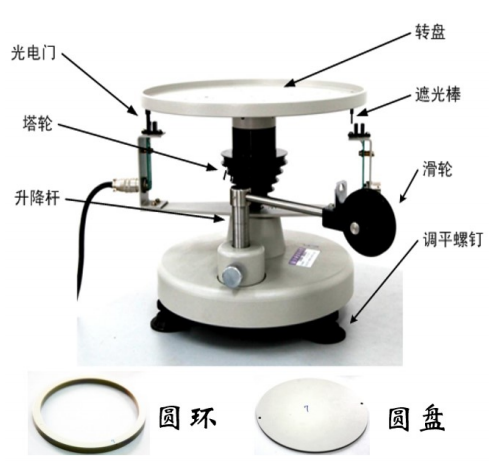
\includegraphics[width=8cm]{apparatus.png}
    \caption{Experimental Setup}
\end{figure}
The multifunctional timer generates an impulse each time the stick passes through the gate of the sensor. It allows measurements with maximum uncertainty of $0.0001s$. It starts the measurement after the first impulse from the sensor, and recording the time used between each pass, thus measuring the time change of certain interval to calculate the angular acceleration.\par
The mass of test samples and the weight was measured by an electronic scale with maximum uncertainty 0.1g.\par
The size of the test samples, the diameter of the cone pulley, and the distance of the changing rotation axis was determined by using a Vernier Caliper with maximum uncertainty 0.02 mm. 

%---------------------------------------------------------------------
%SECTION 3
%---------------------------------------------------------------------

\section{Measurement}

\subsection{Mass measurement}
Measure the mass of the weight and test samples. For convenience, we measure the weight for cirque by measuring the weight of disk 
and the weight of the combination of disk and cirque, then use calculation to yield the certain mass.

\subsection{Length Measurement}
Use Vernier Caliper to measure the size of sample test and the cone pulley. Measure six times for each and take the average value.

\subsection{Time measurement}
Before starting measurements, the power supply was turned on.
\begin{enumerate}
    \item  Through observing a bubble, change the height of the device feet to make the platform level
    \item  Choose the multi-pulse mode and channel A to prepare for the recording
    \item  Click start to begin recording the time measurement data
    \item  Wait for the platform to go 8 round and get 16 data ($T_{01}$-$T_{16}$)
    \item  Click pause to stop and read the recorded time through the screen
    \item  Tie the heavy object on the pulley, make sure the rope is horizontal and won't touch the hole on the roll
    \item  Click start immediately after letting the weight go
    \item Click pause when the weight about to hit the ground
    \item  Record 8 data ($T_{01}$-$T_{08}$) from the screen
\end{enumerate}\par
The above measurement of the rotating period was repeated four times (empty platform, platform with disk, platform with cirque and platform with cylinders). The obtained data is presented 
in Result.\par


%----------------------------------------------------------------------------------------
%	SECTION 4
%----------------------------------------------------------------------------------------
\section{Results}

\subsection{Mass and Length}
The length was measured in the procedure described in 3.2. Because of the hardness of measuring the radius, I measure the diameter first.The diameter equals to $$D=\frac{1}{6}\sum_{i=1}^{6}D_i$$  and the radius equals to  $\frac{D}{2}$. Followed is all the length data. \par
\begin{table}[htbp]
    \centering
    \begin{tabular}{|c|c|c|c|c|c|c|c|}
        \hline
        \multicolumn{6}{|c|}{Length$[mm]\pm0.01[mm]$}&\multicolumn{2}{|c|}{Length$[mm]\pm0.02[mm]$}\\
        \hline
        $R_{c,i}$&$R_{c,o}$&$R_d$&$R_A$&$R_B$&$R$&$d_i$&$d_o$\\ 
        \hline
        149.99&119.93&119.94&14.99&15.00&25.07&~~~~69.95~~~~~&80.11\\
        \hline
    \end{tabular}
    \caption{Length Measurement Data}
\end{table} \par
A simple measurement described in 3.1 yields that the mass is as followed
\begin{table}[H]
    \centering
    \begin{tabular}{|c|c|c|c|}
        \hline
        \multicolumn{4}{|c|}{mass$[g]\pm 0.1[g]$}\\
        \hline
        $m$ & \multicolumn{3}{c|}{54.5}\\ 
        \hline
        $m_d$&488.5&$m_c+m_d$&887.6\\
        \hline
        $m_A$ & 165.8 & $m_B$ & 165.8\\
        \hline
    \end{tabular}
    \caption{Mass Measurement Data}
\end{table} \par



\subsection{Moment of Inertia}

The moment of inertia can be calculated by Eq.1 mentioned in Introduction. The angular accelerations were calculated through making the figures for fitting quadratic curve. I choose Origin2020b to calculate the conic coefficient. Time measured as 3.3 mentioned is the x-axis and degree is the y-axis. The firgures are in the appendix.

\subsubsection{Empty Platform}

 The angular acceleration for the empty platform is $-0.0770\pm 4\times 10^-4rad/s^2$ (the angular acceleration is $2\cdot B_2$ according to the Eq.1). The angular acceleration after hanging the weight is $1.6738\pm4.1\times 10^-3 rad/s^2$. According to Eq.2
$$I_p=\frac{mR(g-R\alpha_2)}{\alpha_2-\alpha_1}=7.6 \times 10^-3\pm 0.0148kg\cdot m^2$$

\subsubsection{Platform with Cirque}

We can find that the platform with cirque at first have the angular acceleration $-0.0502\pm 6\times 10^-4rad/s^2$. The angular acceleration after hanging the weight is $1.1362\pm 2.4\times 10^-3rad/s^2$. According to Eq.1 $$I_p+I_c=\frac{mR(g-R\alpha_2)}{\alpha_2-\alpha_1}=11.2\times 10^-3\pm 0.0218kg\cdot m^2$$ Applying Eq.3, we can find the moment of inertia for the cirque is $3.6\times 10^-3\pm 0.0263kg\cdot m^2$

\subsubsection{Platform with Disk}

We can find that the platform with disk at first have the angular acceleration $-0.0567\pm 2\times 10^-4rad/s^2$. The angular acceleration after hanging the weight is $1.3247\pm 2.7 \times 10^-3rad/s^2$. According to Eq.1 $$I_p+I_d=\frac{mR(g-R\alpha_2)}{\alpha_2-\alpha_1}=9.6 \times 10^-3\pm 0.0187kg\cdot m^2$$ Applying Eq.3, we can find the moment of inertia for the disk is $2.0\times 10^-3\pm 0.0238kg\cdot m^2$

\subsubsection{Platform with cylinders}

We can find that the platform with cylinders at first have the angular acceleration $-0.0652\pm 2\times 10^-4rad/s^2$. The angular acceleration after hanging the weight is $1.5759\pm 4.5\times 10^-3rad/s^2$. According to Eq.1 $$I_p+I_{cy}=\frac{mR(g-R\alpha_2)}{\alpha_2-\alpha_1}=8.1 \times 10^-3\pm 0.0158kg\cdot m^2$$ Applying Eq.3, we can find the moment of inertia for the cylinders is $0.5\times 10^-3\pm 0.0216kg\cdot m^2$.

%----------------------------------------------------------------------------------------
%	SECTION 5
%----------------------------------------------------------------------------------------

\section{Conclusions and Discussion}

\subsection{Moment of Inertia}
According to 3.2, the inside and outside diameter for the cirque seperately equals to $209.98\pm0.03mm$ and $239.92\pm0.06mm$. So, the radius equals to $104.99\pm0.01mm$ and $119.96\pm0.03mm$. A simple measurement described in 3.1 yields that the mass of the cirque equals to $399.1\pm0.1g$. By applying calculus to the mass point's moment of inertia formula, we can find the moment of inertia for the cirque. $$I_c=\frac{1}{2}m({R_{c,i}}^2+{R_{c,o}}^2)=5.071\times 10^-3\pm 2.420\times 10^-3kg\cdot m^2$$ \par

Similarily, the radius of the disk equals to $\frac{D_{d,n}}{2}=119.94\pm0.01mm$, and the mass of the disk equals to $488.5\pm0.1g$. The moment of inertia for the disk ca be found. $$I_d=\frac{1}{2}m{R_d}^2=3.513\times 10^-3\pm 9.28\times 10^-4 kg\cdot m^2$$. \par

The relative difference for the cirque is $28.2\%$ and for the disk is $41.8\%$. Both of them are too large.\par 

But when we turn to the absolute difference. They are similar.One is $1.43\times 10^-3kg\cdot m^2$ and another is$1.47\times 10^-3kg\cdot m^2$. This may show that there exists certain mistake in the measure of the moment inertia for the empty platform. After adding $1.45\times 10^-3kg\cdot m^2$($\frac{1}{2}(1.47+1.43)$) to each, the relative differrence can be decreased to $0.4\%$ and $0.6\%$. But we can not sure since there only exists two groups of data, we still need to turn to the cylinder data to further confirm this hypothesis.

If this hypothesis is true means that platform's theoratical moment of inertia is smaller than the practical measurement data. It may because of the string tied on the weight is not level or touch the hole at some time. These may cause the decrease of the force arm, thus lessening the angular acceleration. And finally the moment of inertia is bigger than the theoratical value.\par

As the fundemental of the measurement, I think that the moment of inertia for the empty platform should be measured several times to decrease the uncertainty. \par

In the lab period, I found that the cirque and the disk cannot fit the platform well, so I have to manually make the rotational axises at the same line often. If other students did not pay attention to it may cause the practical value larger than actual. So, the apparatus can somehow improved by providing a method to fix the position of test samples.

\subsection{Parallel-Axis Theorem}

According to 3.2, the diameter for cylinder A and B seperately equal to $29.98\pm0.03mm$and$30.01\pm0.02mm$. So, the radius equals to $14.99\pm0.02mm$ and $15.00\pm0.01mm$. A simple measurement described in 3.1 yields that the mass of two cylinders both equals to $165.8\pm0.1g$. By applying calculus to the mass point's moment of inertia formula, we can find that the moment of inertia for each cylinder euqals $$I_A=\frac{1}{2}m{R_{A}}^2=1.9\times 10^-5\pm 4.4\times 10^-5kg\cdot m^2$$$$I_B=\frac{1}{2}m{R_{B}}^2=1.9\times 10^-5\pm 3.2\times 10^-5kg\cdot m^2$$\par
We could calculate distance required in theorem through measure both the inner distance $d_i$ and outer distance $d_o$ and find the average $\frac{d_i+d_o}{2}$. The distance we got is $75.03mm\pm 0.01mm$.\par 
Applying the Parallel-Axis Theorem, we can find that the total moment of inertia for the cylinder system equals $1.9\times 10^-3\pm 9.44\times 10^-4kg\cdot m^2$. It has a huge relative difference that is $74.2\%$. But after adding $1.45\times 10^-3kg\cdot m^2$, which was mentioned in the formal hypothesis, the relative difference is only $2.1\%$. The theoratical and practical value is almost the same. So the parallel-axis theorem can be somehow proved. \par 
But I think only one group of data is not enough to prove the parallel-axis theorem. There exists 5 different distancecs to fix cylinders in 4 different directions, many other datas can be measured to further prove the parallel-axis theorem.

\section{Reference}
Xiner Shen, Neale Haugen, Exercise 1, Moment of Inertia

\newpage
{\LARGE\textbf{APPENDIX}}
\setcounter{section}{0}
\renewcommand\thesection{\Alph{section}}

\section {Measurement Uncertainty Analysis}

\subsection{Uncertainty of the mass}

The uncertainty of the mass mainly caused by the apparatus. The electronic scale has the type-B uncertainty $0.1g$.\par

\subsection{Uncertainty of the length}

The uncertainty of the mass mainly caused by the apparatus. The electronic scale has the type-B uncertainty $0.02mm$.\par

In order to decrease the uncertainty caused by manual measurement, those length values were measured six times \par 

$$\sigma=\sqrt{\frac{\sum_{i=1}^n(x_i-\overline{x})^2}{n-1}}$$ \par

\newcommand{\tabincell}[2]{\begin{tabular}{@{}#1@{}}#2\end{tabular}}

\begin{table}[htbp]
    \begin{center}
        \begin{tabular}{|c|c|c|c|c|c|c|}
            \hline
            \multicolumn{7}{|c|}{length[mm]$\pm$0.02[mm]} \\
            \hline
             & 1 & 2 & 3 & 4 & 5 & 6 \\
            \hline
            $D_{c,i}$ & 209.98 & 209.96 & 210.00 & 209.98 & 210.00 & 209.94 \\
            \hline
            $D_{c,o}$ & 239.92 & 240.04 & 239.86 & 239.90 & 239.98 & 239.96 \\
            \hline
            $D_d$ & 239.84 & 239.86 & 239.90 & 239.82 & 239.86 & 239.88 \\ 
            \hline
            $D_A$ & 29.92 & 29.98 & 30.00 & 29.98 & 29.96 & 30.02 \\
            \hline
            $D_B$ & 30.02 & 29.98 & 30.04 & 29.98 & 30.00 & 30.02 \\
             \hline
            $R$ & 50.10 & 50.18 & 50.16 & 50.18 & 50.14 & 50.12 \\
            \hline
            $d_i$ & 69.98 & 69.90 & 69.98 & 69.94 & 69.96 & 69.94 \\
            \hline
            $d_o$ & 80.10 & 80.06 & 80.10 & 80.16 & 80.12 & 80.14 \\
             \hline   
        \end {tabular}
        \caption{Length Measurement Data}
     \end {center}
\end{table}

\begin{table}[H]
    \begin{tabular}{|c|c|c|c|c|}
        \hline
        & \tabincell{c}{Cirque\\Inner Diameter} &\tabincell{c}{Cirque\\Outer Diameter} & \tabincell{c}{Disk Diameter} & \tabincell{c}{Cylinder A\\Diameter} \\
        \hline
        Mean(mm) & 209.98 & 239.92 & 239.88 & 29.98 \\
        \hline
        \tabincell{c}{Uncertainty\\(mm)} & 0.03 & 0.06 & 0.03 & 0.03 \\
        \hline
        & \tabincell{c}{Cylinder B\\Diameter} & \tabincell{c}{Cone Pulley\\Diameter} & \tabincell{c}{Inner Axis\\Movement Distance} & \tabincell{c}{Outer Axis\\Movement Distance}\\
        \hline
        Mean(mm) & 30.00 & 50.15 & 69.95 & 80.11\\
        \hline
        \tabincell{c}{Uncertainty\\(mm)} & 0.02 & 0.03 & 0.03 & 0.04\\
        \hline
    \end{tabular}
    \caption{The Mean and Uncertainty of Length Measurement Data}
\end{table}

\begin{figure}[h]
    \centering
    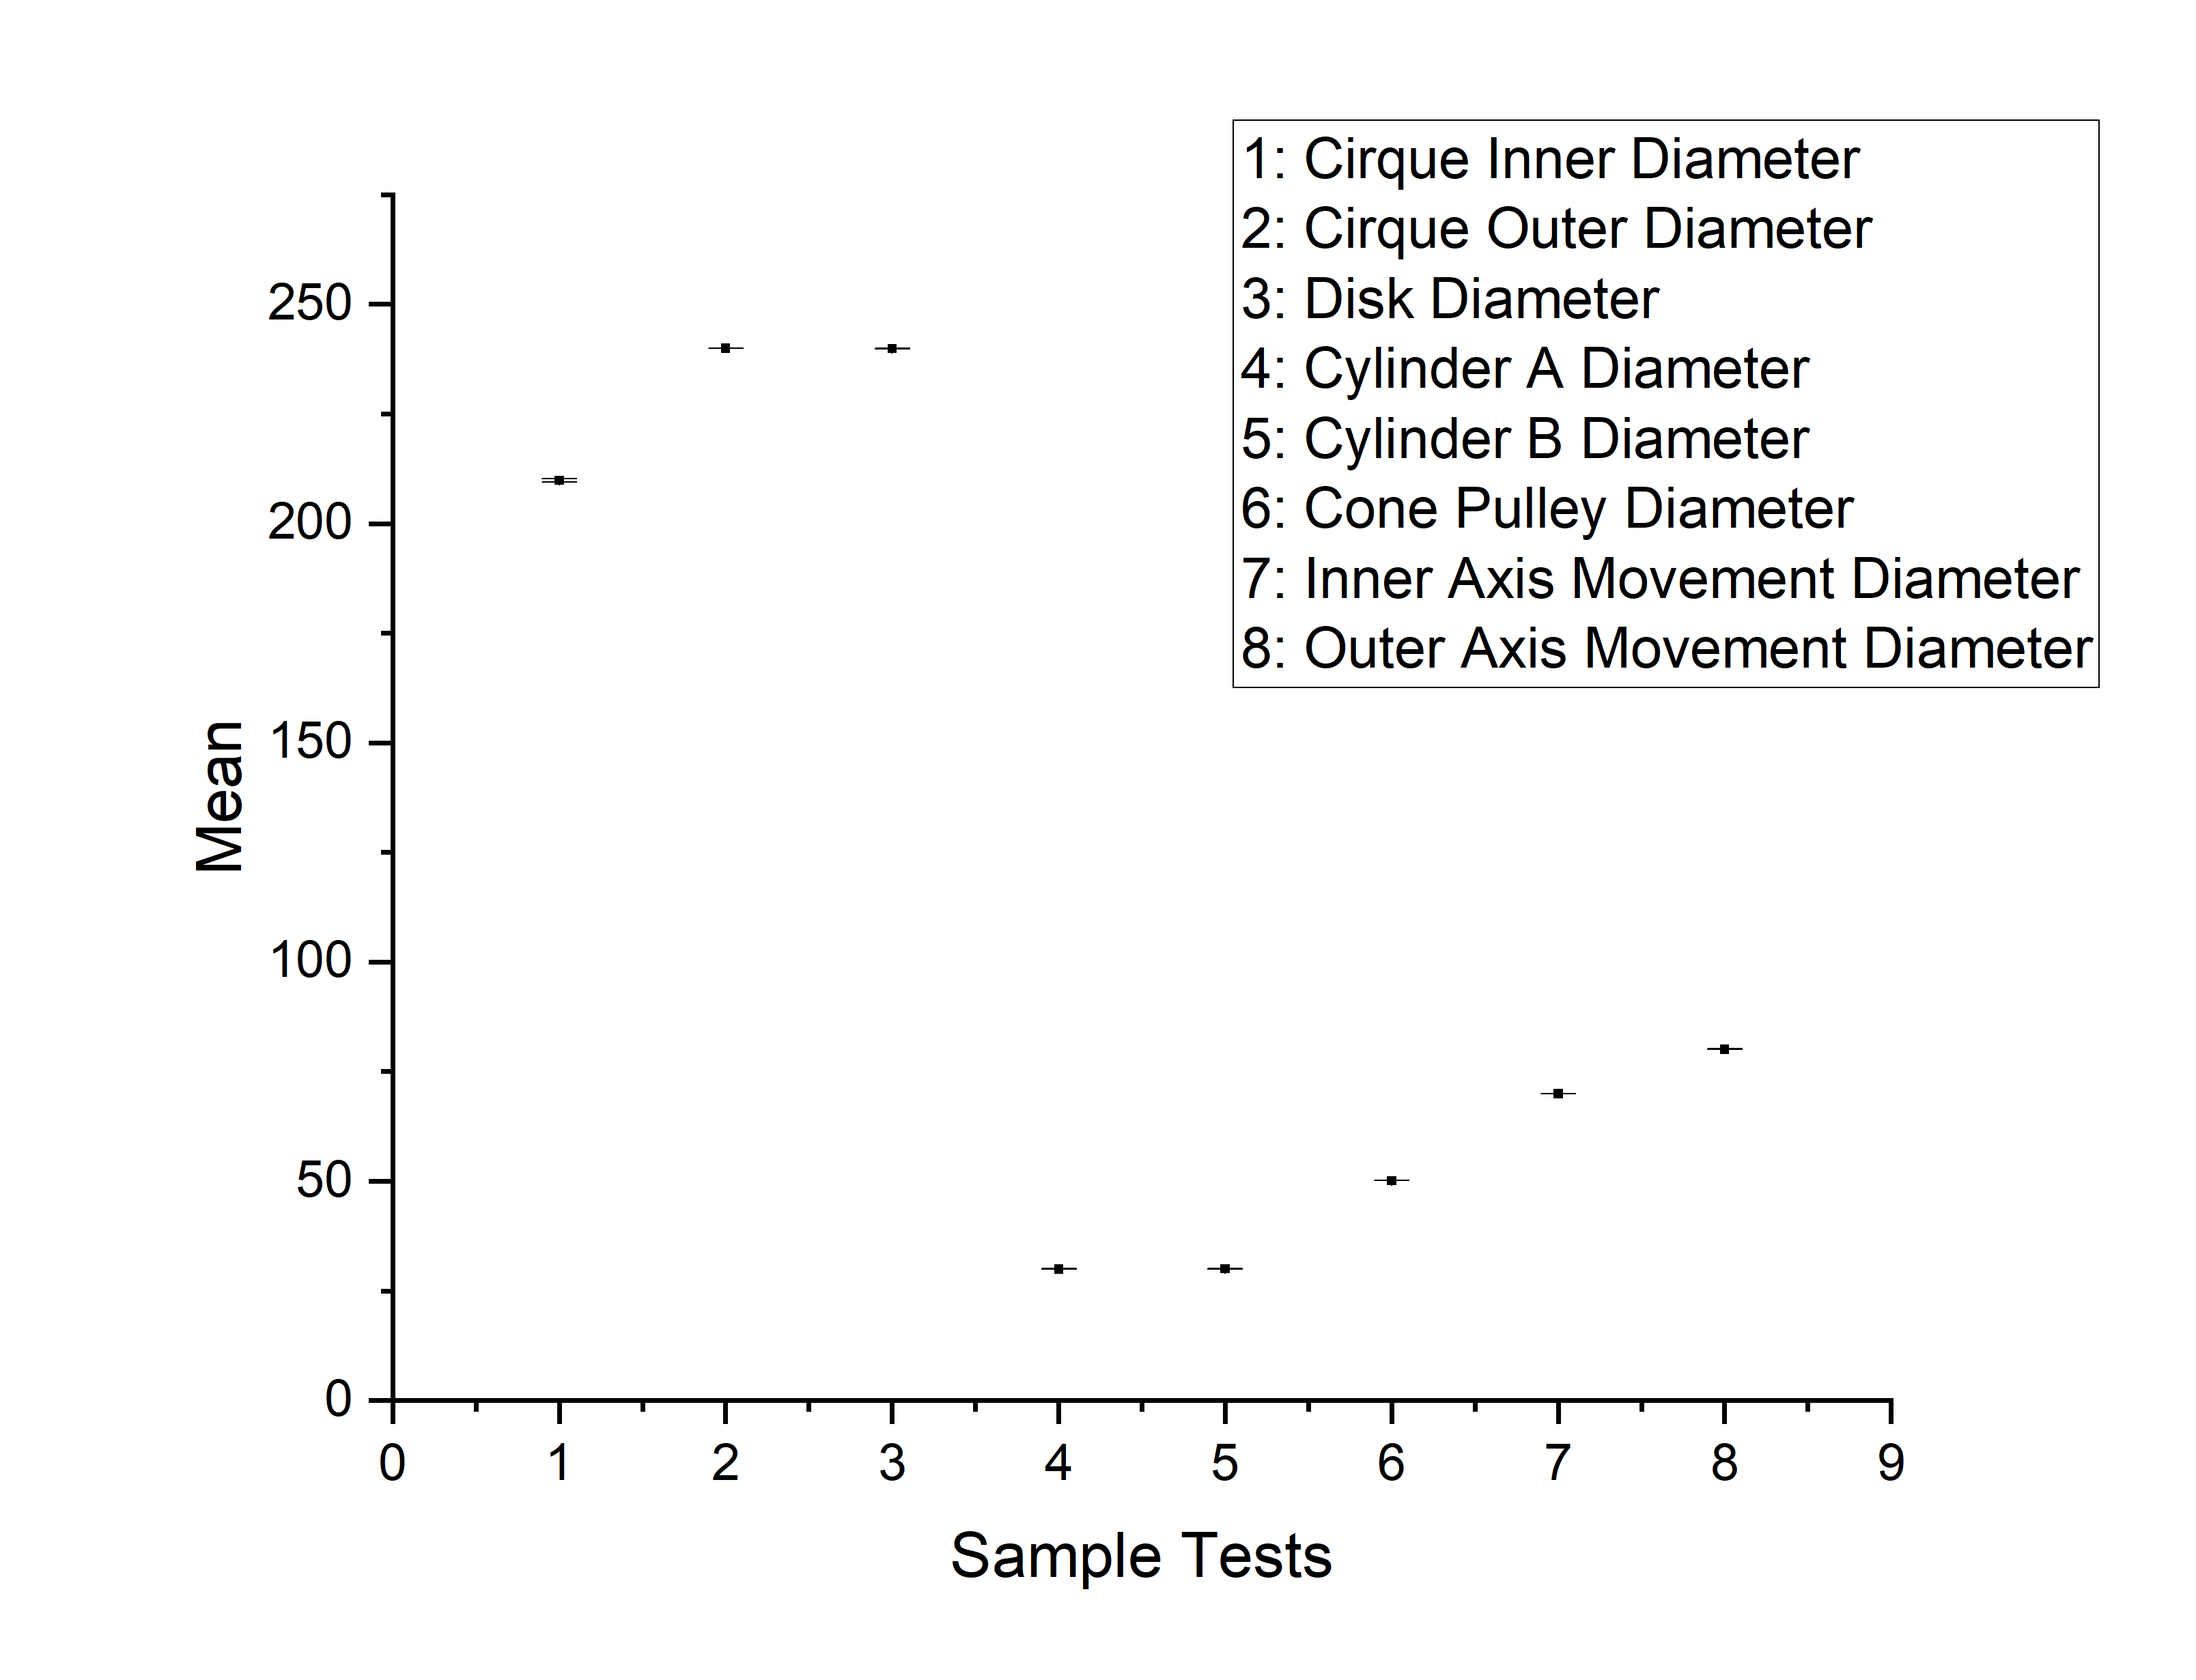
\includegraphics[width=13cm]{uncertainty.png}
    \caption{Uncertainty of Length}
\end{figure}



\subsection{The Calculation Uncertianty}
\subsubsection{The Angular Acceleration Uncertainty}
The formation to descript the relationship between degree and angular acceleration is $\theta_m=km\pi=\omega_0t_m+\frac{1}{2}\alpha{t_m}^2$. So $$\sigma_\alpha=\sqrt{{(\frac{\partial_{\theta_m}}{\partial_\alpha}})^2{\sigma_{B_2}}^2}=2\sigma_{B_2}$$ $\sigma_{B_2}$ is calculated automatically by Origin2020b.

\subsubsection{the Superposition Theorem Uncertainty}
The formation to descript the relationship between the moment of inertia for the system and for seperate objects, $I_3=I_1+I_2$.

$$\sigma_{I_3}=\sqrt{(\frac{\partial_{I_3}}{\partial_{I_1}})^2{\sigma_{I_1}}^2+(\frac{\partial_{I_3}}{\partial_{I_2}})^2{\sigma_{I_2}}^2}=\sqrt{{\sigma_{I_1}}^2+{\sigma_{I_2}}^2}$$

\subsubsection{the Practical Moment of Inertia Uncertainty}
The formation to calculate the moment of inertia is $I=\frac{mR(g-R\alpha_2)}{\alpha_2-\alpha_1}$. So 
$$
\left\{
\begin{aligned}
    &\frac{\partial_I}{\partial_m}=\frac{R(g-R\alpha_2)}{\alpha_2-\alpha_1}\\
    &\frac{\partial_I}{\partial_R}=\frac{m(g-2R\alpha_2)}{\alpha_2-\alpha_1}\\
    &\frac{\partial_I}{\partial_{\alpha_1}}=\frac{mR(g-R\alpha_2)}{(\alpha_2-\alpha_1)^2}\\
    &\frac{\partial_I}{\partial_{\alpha_2}}=\frac{mR(R\alpha_1-g)}{(\alpha2-\alpha1)^2}
\end{aligned}
\right.
$$

$$\sigma_I=\sqrt{(\frac{\partial_I}{\partial_m})^2{\sigma_m}^2+(\frac{\partial_I}{\partial_R})^2{\sigma_R}^2+(\frac{\partial_I}{\partial_{\alpha_1}})^2{\sigma_{\alpha_1}}^2+(\frac{\partial_I}{\partial_{\alpha_2}})^2{\sigma_{\alpha_2}}^2}$$
$$=\sqrt{(\frac{R(g-R\alpha_2)}{\alpha_2-\alpha_1})^2{\sigma_m}^2+(\frac{m(g-2R\alpha_2)}{\alpha_2-\alpha_1})^2{\sigma_R}^2+(\frac{mR(g-R\alpha_2)}{(\alpha_2-\alpha_1)^2})^2{\sigma_{\alpha_1}}^2+(\frac{mR(R\alpha_1-g)}{(\alpha2-\alpha1)^2})^2{\sigma_{\alpha_2}}^2}$$

Through putting the data calculated seperately for empty platform, platform with cirque, platform with disk and platform with cylinders, we can get all the uncertainty for the practical moment of inertia.

$$
\begin{aligned}
{\sigma_{I_p}}^2=&(\frac{\frac{25.07}{1000}\times(9.794-\frac{25.07}{1000}\times 1.6738)}{1.6738-(-0.0770)})^2\times{0.1}^2\\
&+(\frac{\frac{54.5}{1000}\times(9.794-2\times \frac{25.07}{1000}\times 1.6738)}{1.6738-(-0.0770)})^2\times{0.016}^2\\
&+(\frac{\frac{54.5}{1000}\times \frac{25.07}{1000}\times(9.794-\frac{25.07}{1000}\times 1.6738)}{(1.6738-(-0.0770)})^2\times{0.00035362}^2\\
&+(\frac{\frac{54.5}{1000}\times\frac{25.07}{1000}(\frac{25.07}{1000}\times(-0.0770)-9.794)}{(1.6378-(-0.0770))^2})^2\times{0.00410}^2\\
\sigma_{I_p}=&0.0148kg\cdot m^2
\end{aligned}
$$

$$
\begin{aligned}
{\sigma_{I_p}}^2=&(\frac{\frac{25.07}{1000}\times(9.794-\frac{25.07}{1000}\times 1.1362)}{1.1362-(-0.0502)})^2\times{0.1}^2\\
&+(\frac{\frac{54.5}{1000}\times(9.794-2\times \frac{25.07}{1000}\times 1.1362)}{1.1362-(-0.0502)})^2\times{0.016}^2\\
&+(\frac{\frac{54.5}{1000}\times \frac{25.07}{1000}\times(9.794-\frac{25.07}{1000}\times 1.1362)}{(1.1362-(-0.0502)})^2\times{0.00057596}^2\\
&+(\frac{\frac{54.5}{1000}\times\frac{25.07}{1000}(\frac{25.07}{1000}\times(-0.0502)-9.794)}{(1.1362-(-0.0502))^2})^2\times{0.00236}^2\\
\sigma_{I_p+I_c}=&0.218kg\cdot m^2
\end{aligned}
$$

$$
\begin{aligned}
{\sigma_{I_p+I_d}}^2=&(\frac{\frac{25.07}{1000}\times(9.794-\frac{25.07}{1000}\times 1.3247)}{1.3247-(-0.0567)})^2\times{0.1}^2\\
&+(\frac{\frac{54.5}{1000}\times(9.794-2\times \frac{25.07}{1000}\times 1.3247)}{1.3247-(-0.0567)})^2\times{0.016}^2\\
&+(\frac{\frac{54.5}{1000}\times \frac{25.07}{1000}\times(9.794-\frac{25.07}{1000}\times 1.3247)}{(1.3247-(-0.0567)})^2\times{0.00023631}^2\\
&+(\frac{\frac{54.5}{1000}\times\frac{25.07}{1000}(\frac{25.07}{1000}\times(-0.0567)-9.794)}{(1.3742-(-0.0567))^2})^2\times{0.00272}^2\\
\sigma_{I_p+I_d}=&0.0187kg\cdot m^2
\end{aligned}
$$

$$
\begin{aligned}
{\sigma_{I_p+I_cy}}^2=&(\frac{\frac{25.07}{1000}\times(9.794-\frac{25.07}{1000}\times 1.6738)}{1.6738-(-0.0770)})^2\times{0.1}^2\\
&+(\frac{\frac{54.5}{1000}\times(9.794-2\times \frac{25.07}{1000}\times 1.6738)}{1.6738-(-0.0770)})^2\times{0.016}^2\\
&+(\frac{\frac{54.5}{1000}\times \frac{25.07}{1000}\times(9.794-\frac{25.07}{1000}\times 1.5759)}{(1.5759-(-0.0652)})^2\times{0.00024561}^2\\
&+(\frac{\frac{54.5}{1000}\times\frac{25.07}{1000}(\frac{25.07}{1000}\times(-0.0652)-9.794)}{(1.5759-(-0.0652))^2})^2\times{0.00478}^2\\
\sigma_{I_p+I_cy}=&0.0158kg\cdot m^2
\end{aligned}
$$

\subsubsection{the Theoratical Moment of Inertia Uncertainty}
 
    Through applying the calculus on $I=mr^2$. We could find that for disks and cylinders $I_d=I_cy=\frac{1}{2}mR^2$, and for cirques $I_c=\frac{1}{2}m({R_i}^2+{R_o}^2)$.\par
    For cirques, we can find that
    $$
    \begin{aligned}
    \sigma_{I_c}&=\sqrt{(\frac{\partial_{I_c}}{\partial_m})^2{\sigma_m}^2+(\frac{\partial_{I_c}}{\partial_{R_{c,i}}})^2{\sigma_{R_{c,i}}}^2+(\frac{\partial_{I_c}}{\partial_{R_{c,o}}})^2{\sigma_{R_{c,o}}}^2}\\
    &=\sqrt{(\frac{1}{2}(R_{c,i}^2+R_{c,o}^2))^2{\sigma_m}^2+(mR_{c,i})^2{\sigma_{R_{c,i}}}^2+(mR_{c,o})^2{\sigma_{R_{c,o}}}^2}\\
    &=\sqrt{(\frac{1}{2}(\frac{104.99}{1000}^2+\frac{119.96}{1000}^2))^2\times{0.1}^2+(\frac{399.1}{1000}\times\frac{104.99}{1000})^2\times{0.01}^2+(\frac{399.1}{1000}\times\frac{119.96}{1000})^2\times{0.03}^2}\\
    &=2.420\times 10^-3 kg\cdot m^2
    \end{aligned}
    $$
    \par 

    For disks and cylinders, we can find that
    $$
    \begin{aligned}
    \sigma_{I_d}&=\sqrt{(\frac{\partial_{I_d}}{\partial_m})^2{\sigma_m}^2+(\frac{\partial_{I_d}}{\partial_R})^2{\sigma_R}^2}=\sqrt{(\frac{R^2}{2})^2{\sigma_m}^2+(mR)^2{\sigma_R}^2}\\
    &=\sqrt{(\frac{(\frac{119.94}{1000})^2}{2})^2\times{0.1}^2+(\frac{488.5}{1000}\times \frac{119.94}{1000})^2\times{0.014}^2}=9.28\times 10^-4kg\cdot m^2
    \end{aligned}
    $$ 

    $$
    \begin{aligned}
    \sigma_{I_{cy_A}}&=\sqrt{(\frac{\partial_{I_{cy}}}{\partial_m})^2{\sigma_m}^2+(\frac{\partial_{I_{cy}}}{\partial_R})^2{\sigma_R}^2}=\sqrt{(\frac{R^2}{2})^2{\sigma_m}^2+(mR)^2{\sigma_R}^2}\\
    &=\sqrt{(\frac{(\frac{14.99}{1000})^2}{2})^2\times{0.1}^2+(\frac{165.8}{1000}\times \frac{14.99}{1000})^2\times{0.017}^2}=4.4\times 10^-5kg\cdot m^2
    \end{aligned}
    $$ 

    $$
    \begin{aligned}
    \sigma_{I_{cy_B}}&=\sqrt{(\frac{\partial_{I_{cy}}}{\partial_m})^2{\sigma_m}^2+(\frac{\partial_{I_{cy}}}{\partial_R})^2{\sigma_R}^2}=\sqrt{(\frac{R^2}{2})^2{\sigma_m}^2+(mR)^2{\sigma_R}^2}\\
    &=\sqrt{(\frac{(\frac{15.00}{1000})^2}{2})^2\times{0.1}^2+(\frac{165.8}{1000}\times \frac{15.00}{1000})^2\times{0.012}^2}=3.2\times 10^-5kg\cdot m^2
    \end{aligned}
    $$ 

\subsubsection{The Parallel-Axis Theorem Uncertainty}
The parallel-axis theorem is $I_p=I_{cm}+Md^2$.

$$
\begin{aligned}
\sigma_{I_p}&=\sqrt{(\frac{\partial_{I_p}}{\partial_M})^2{\sigma_M}^2+(\frac{\partial_{I_c}}{\partial_{d}})^2{\sigma_{d}}^2+(\frac{\partial_{I_p}}{\partial_{I_{cm}}})^2{\sigma_{I_{cm}}}^2}=\sqrt{(d^2)^2{\sigma_M}^2+(2Md)^2{\sigma_{d}}^2+(1)^2{\sigma_{I_{cm}}}^2}\\
&=\sqrt{((\frac{75.03}{1000})^2)^2\times{0.014}^2+(2\times\frac{331.6}{1000}\times\frac{75.03}{1000})^2\times{0.0104}^2+{5.44\times 10^-5}^2}\\
&=9.44\times 10^-4 kg\cdot m^2
\end{aligned}
$$

\section{Data Sheet}
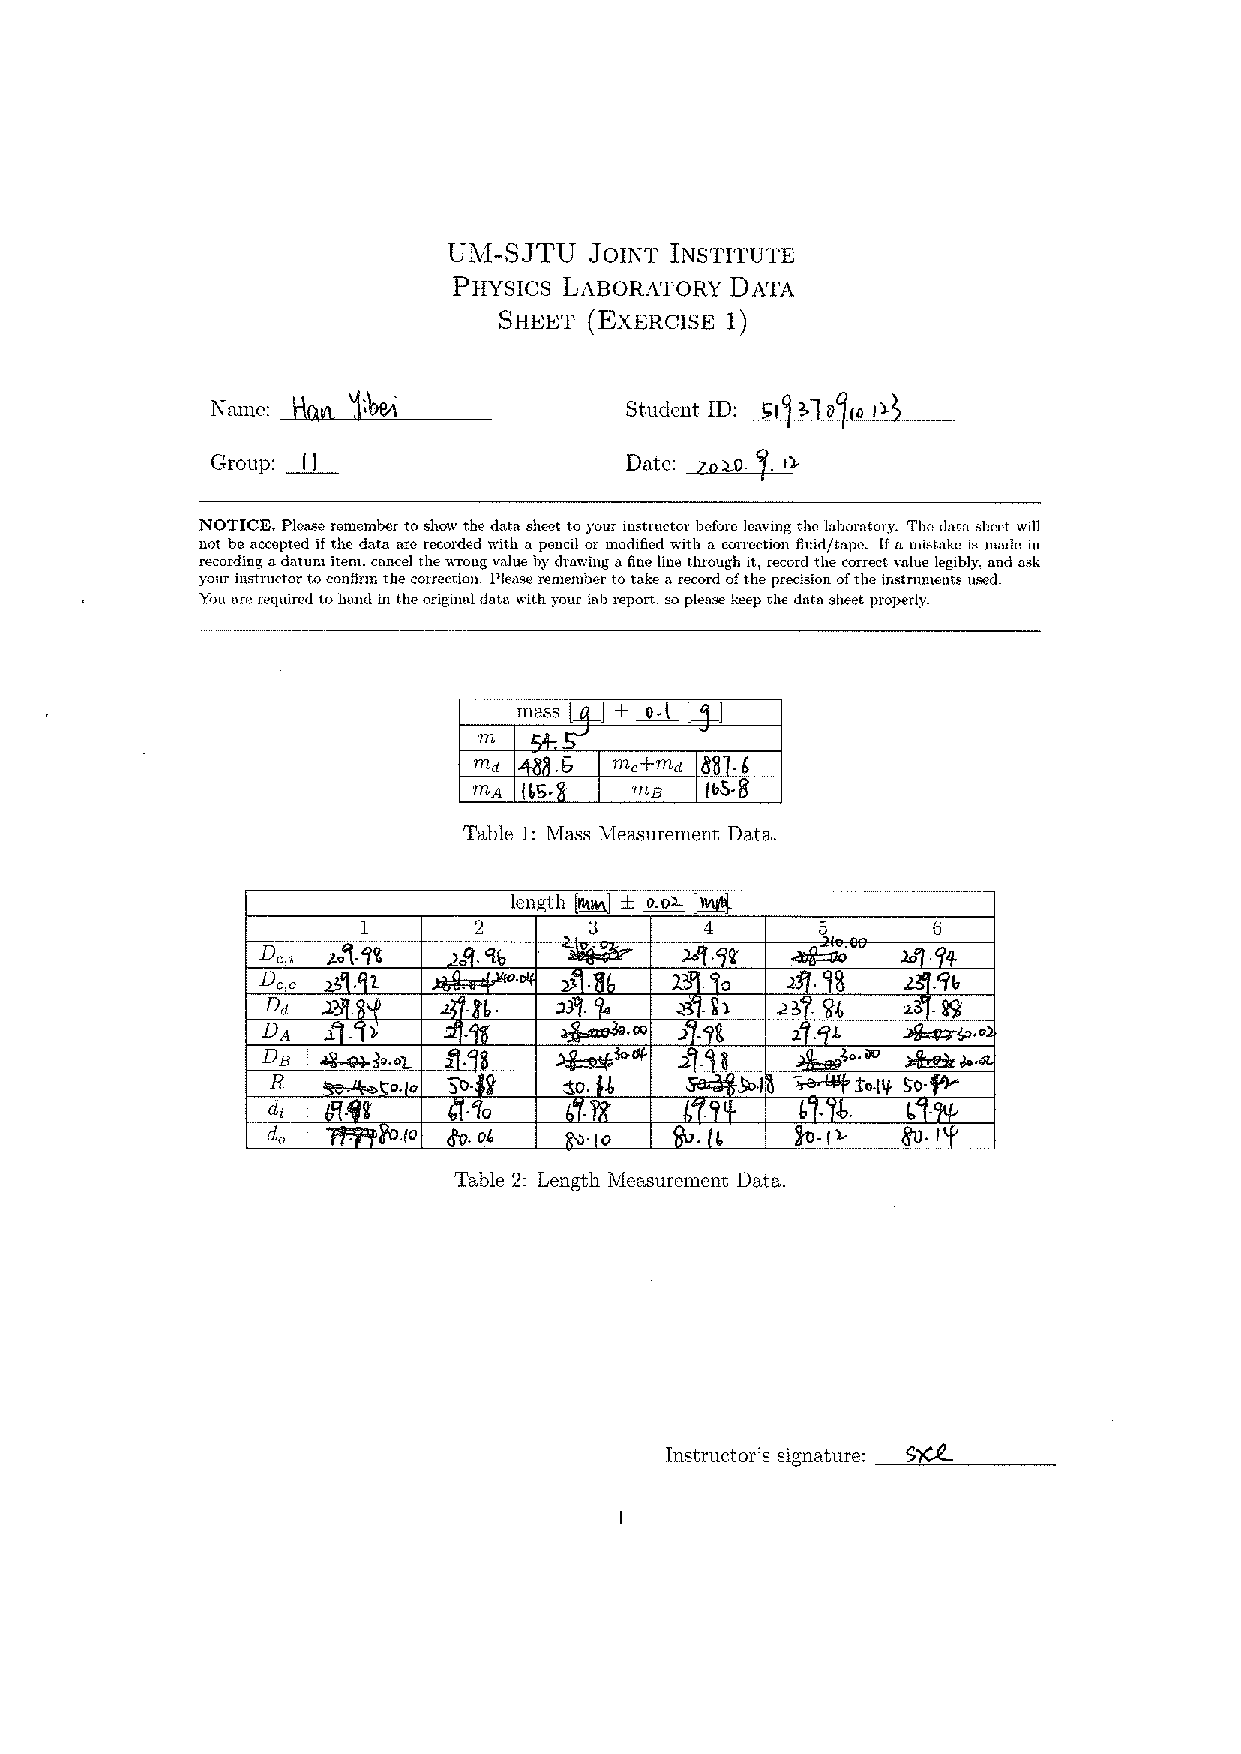
\includepdf[pages={1,2,3,4,5}]{datasheet.pdf}

\section{Supporting Information}

\begin{figure}[h]
    \centering
    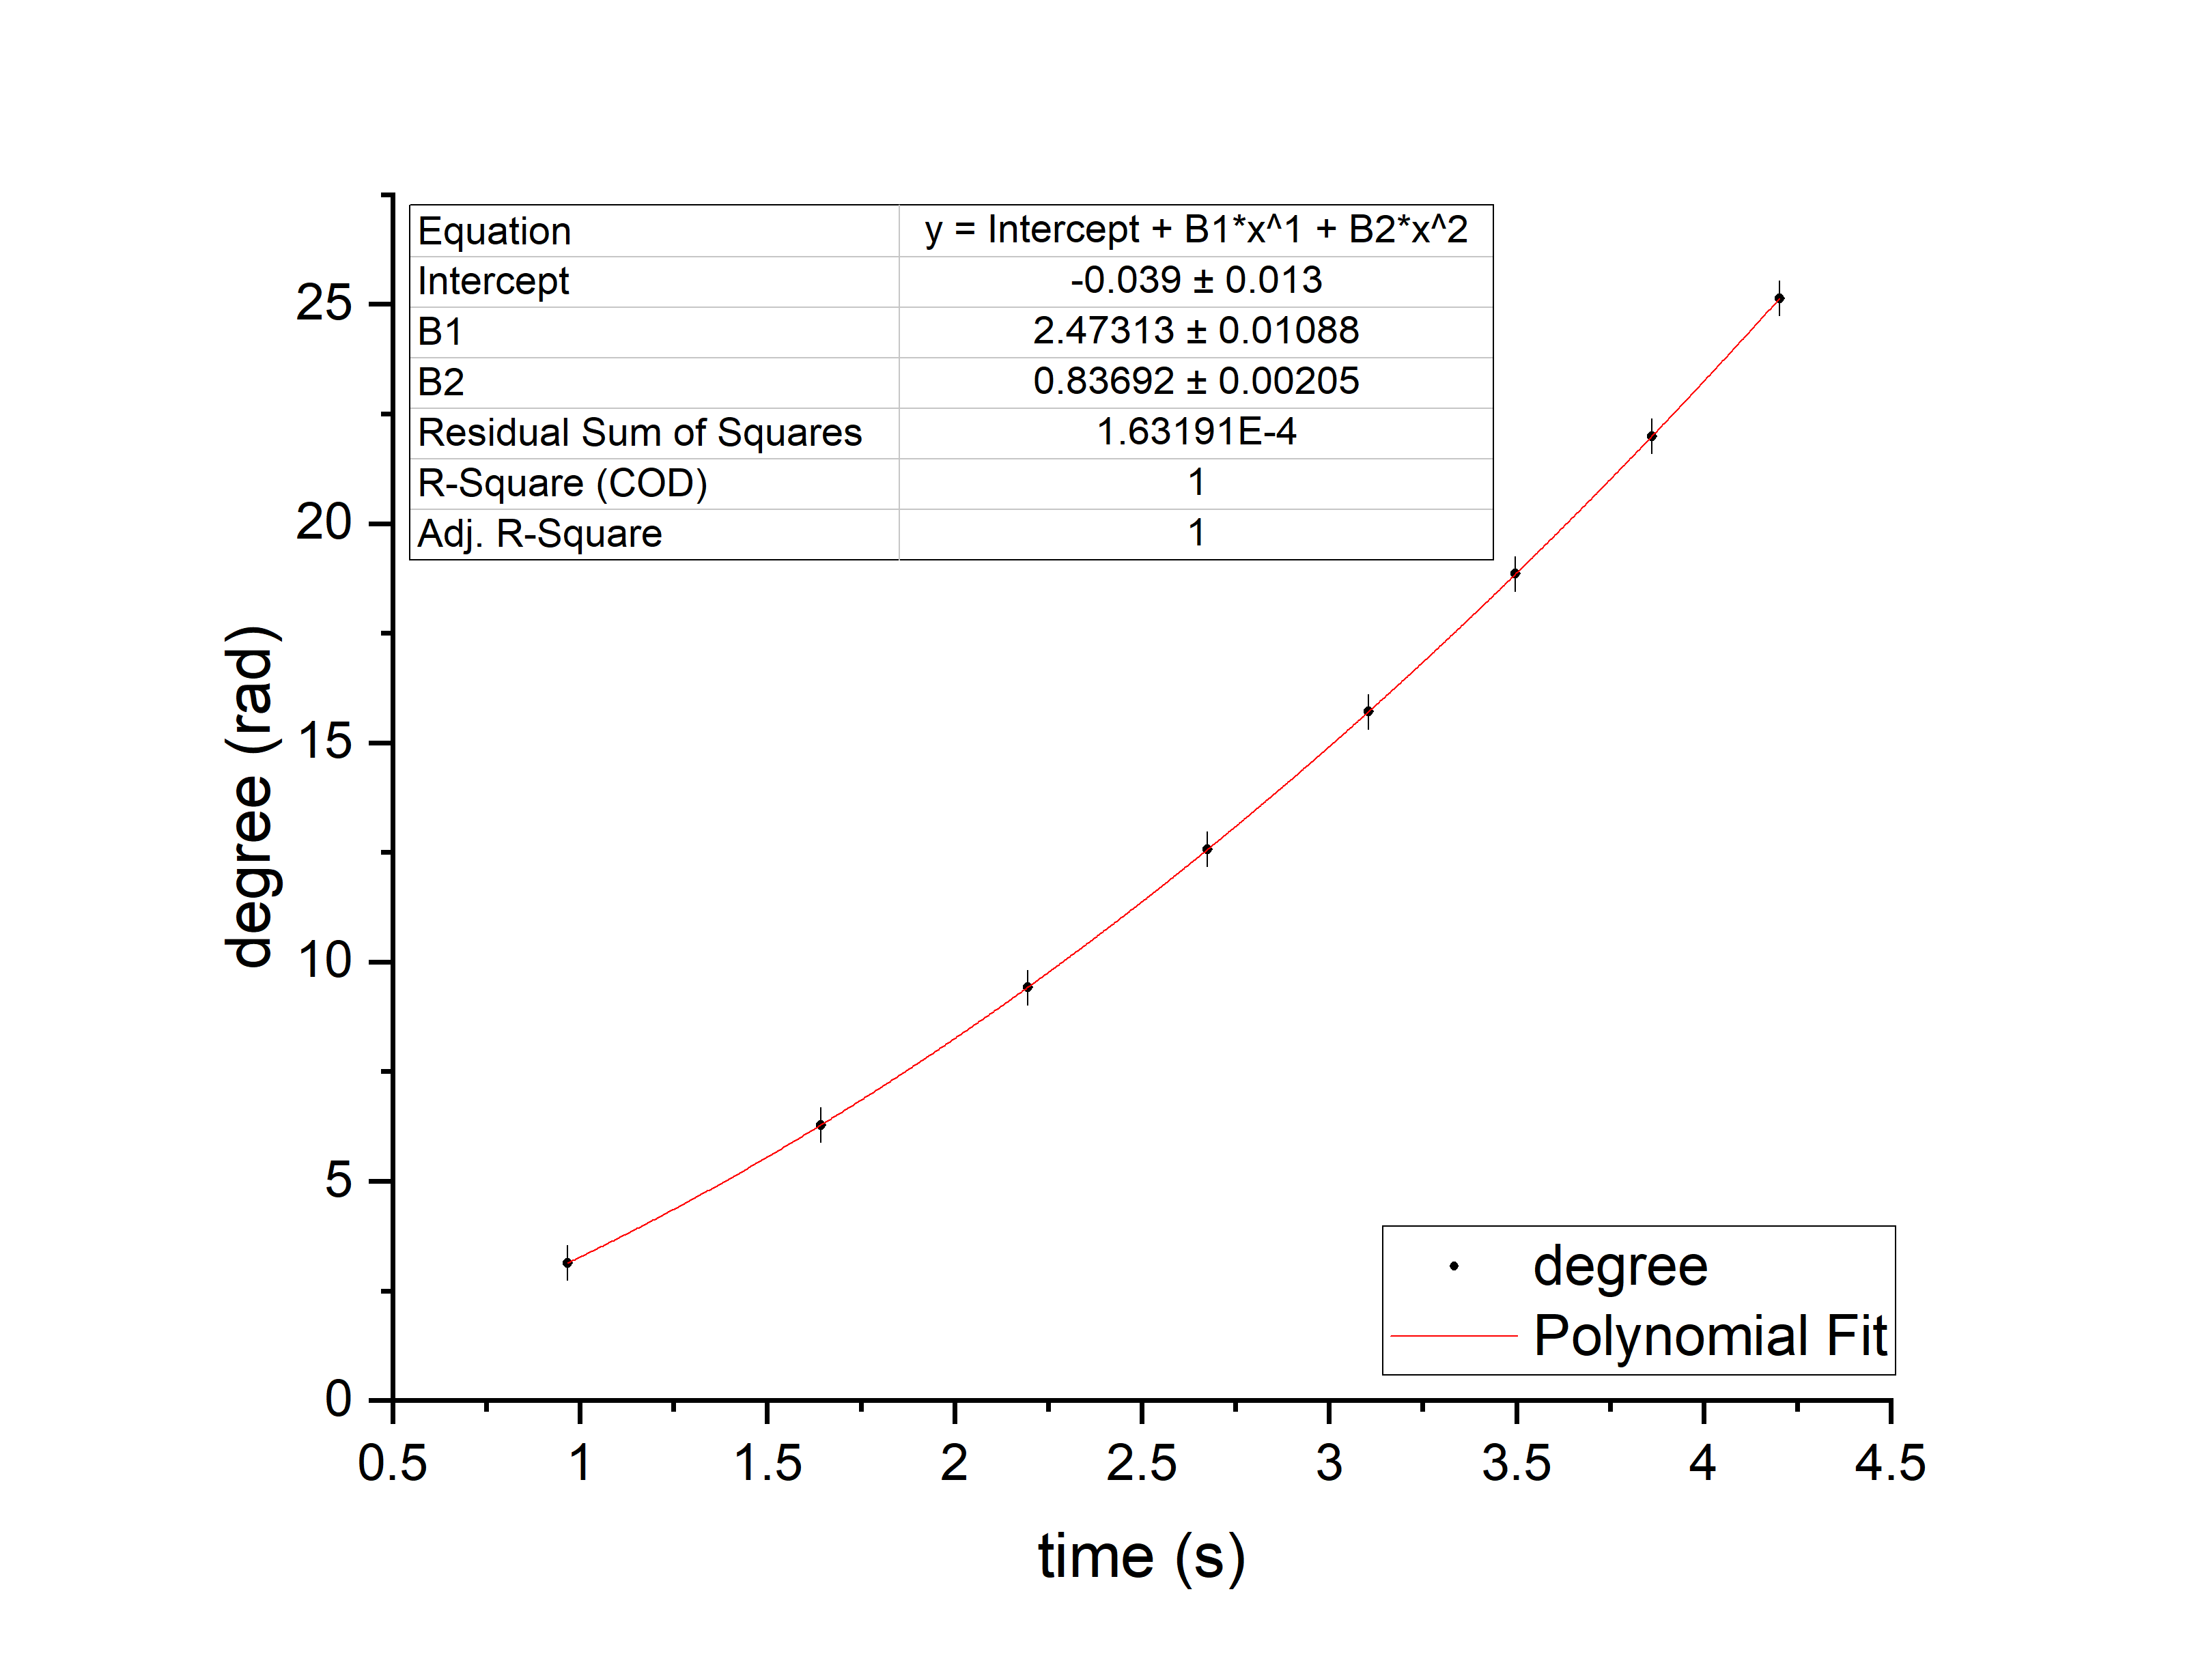
\includegraphics[width=10cm]{emptyw.png}
    \caption{Time Measurement Data for Empty Platform without weight}
\end{figure}

\begin{figure}[h]
    \centering
    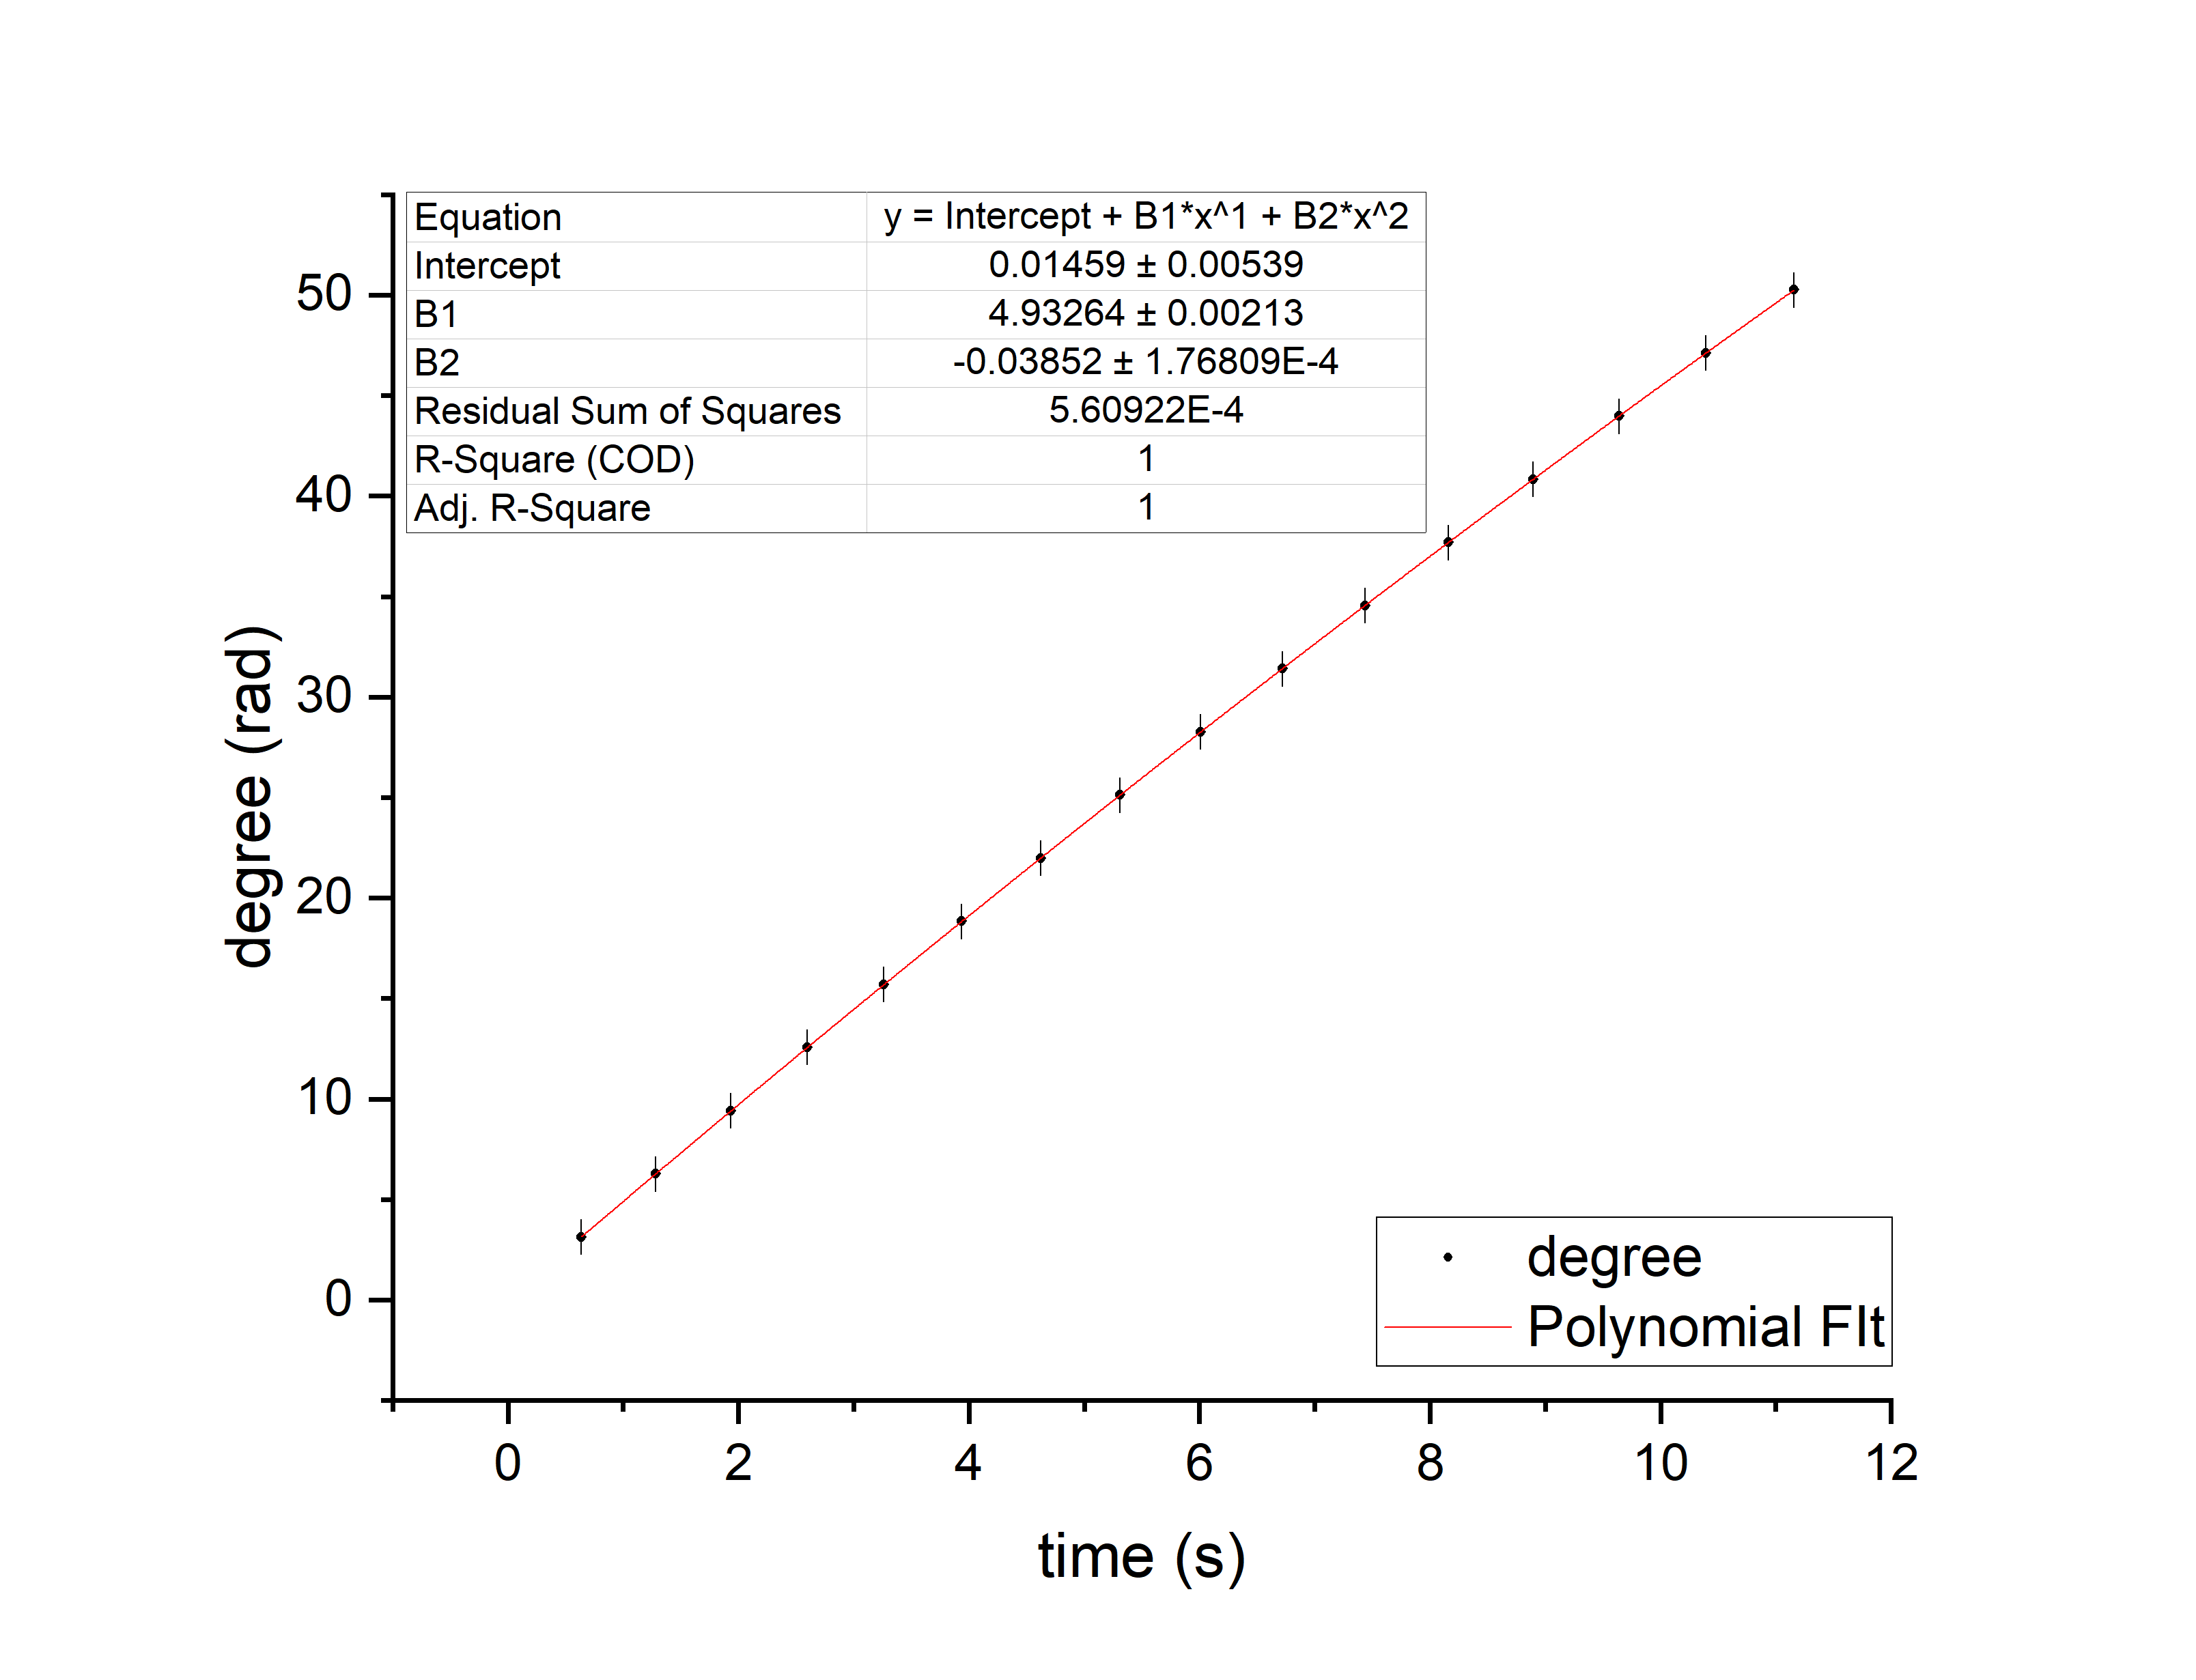
\includegraphics[width=10cm]{emptywo.png}
    \caption{Time Measurement Data for Empty Platform with weight}
\end{figure}

\begin{figure}[h]
    \centering
    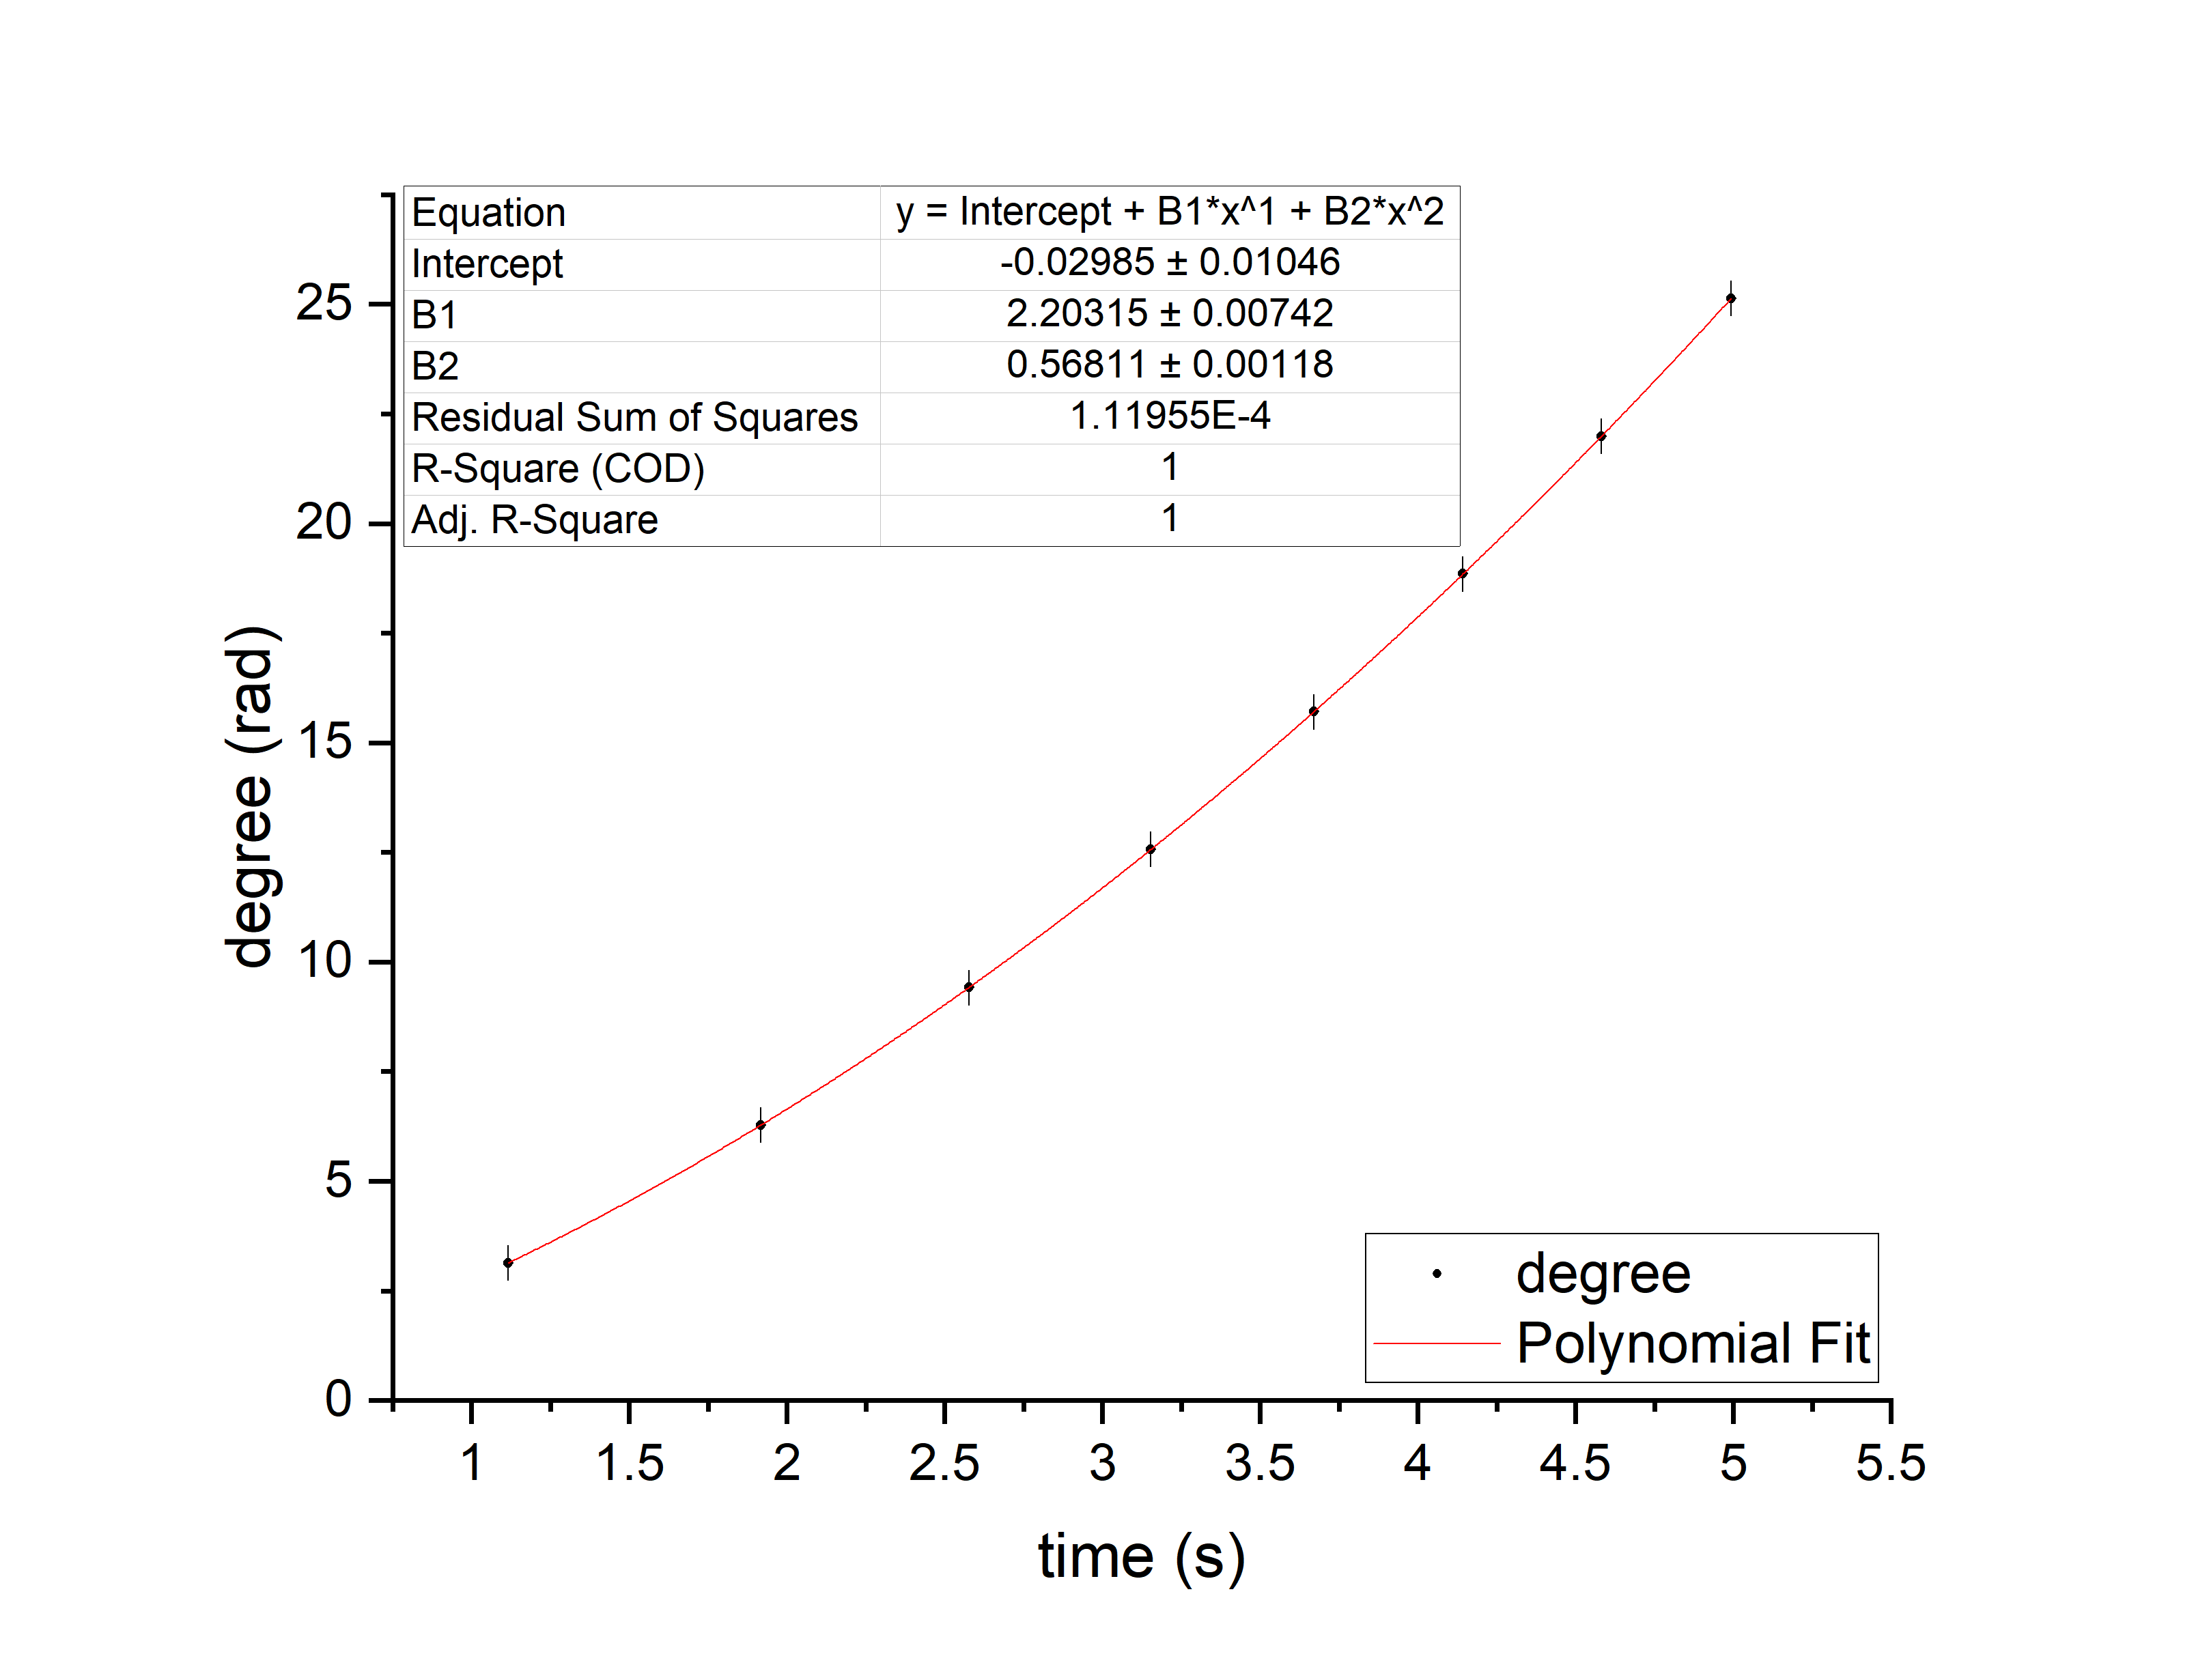
\includegraphics[width=12cm]{cirquew.png}
    \caption{Time Measurement Data for Platform with Cirque but without weight}
\end{figure}

\begin{figure}[h]
    \centering
    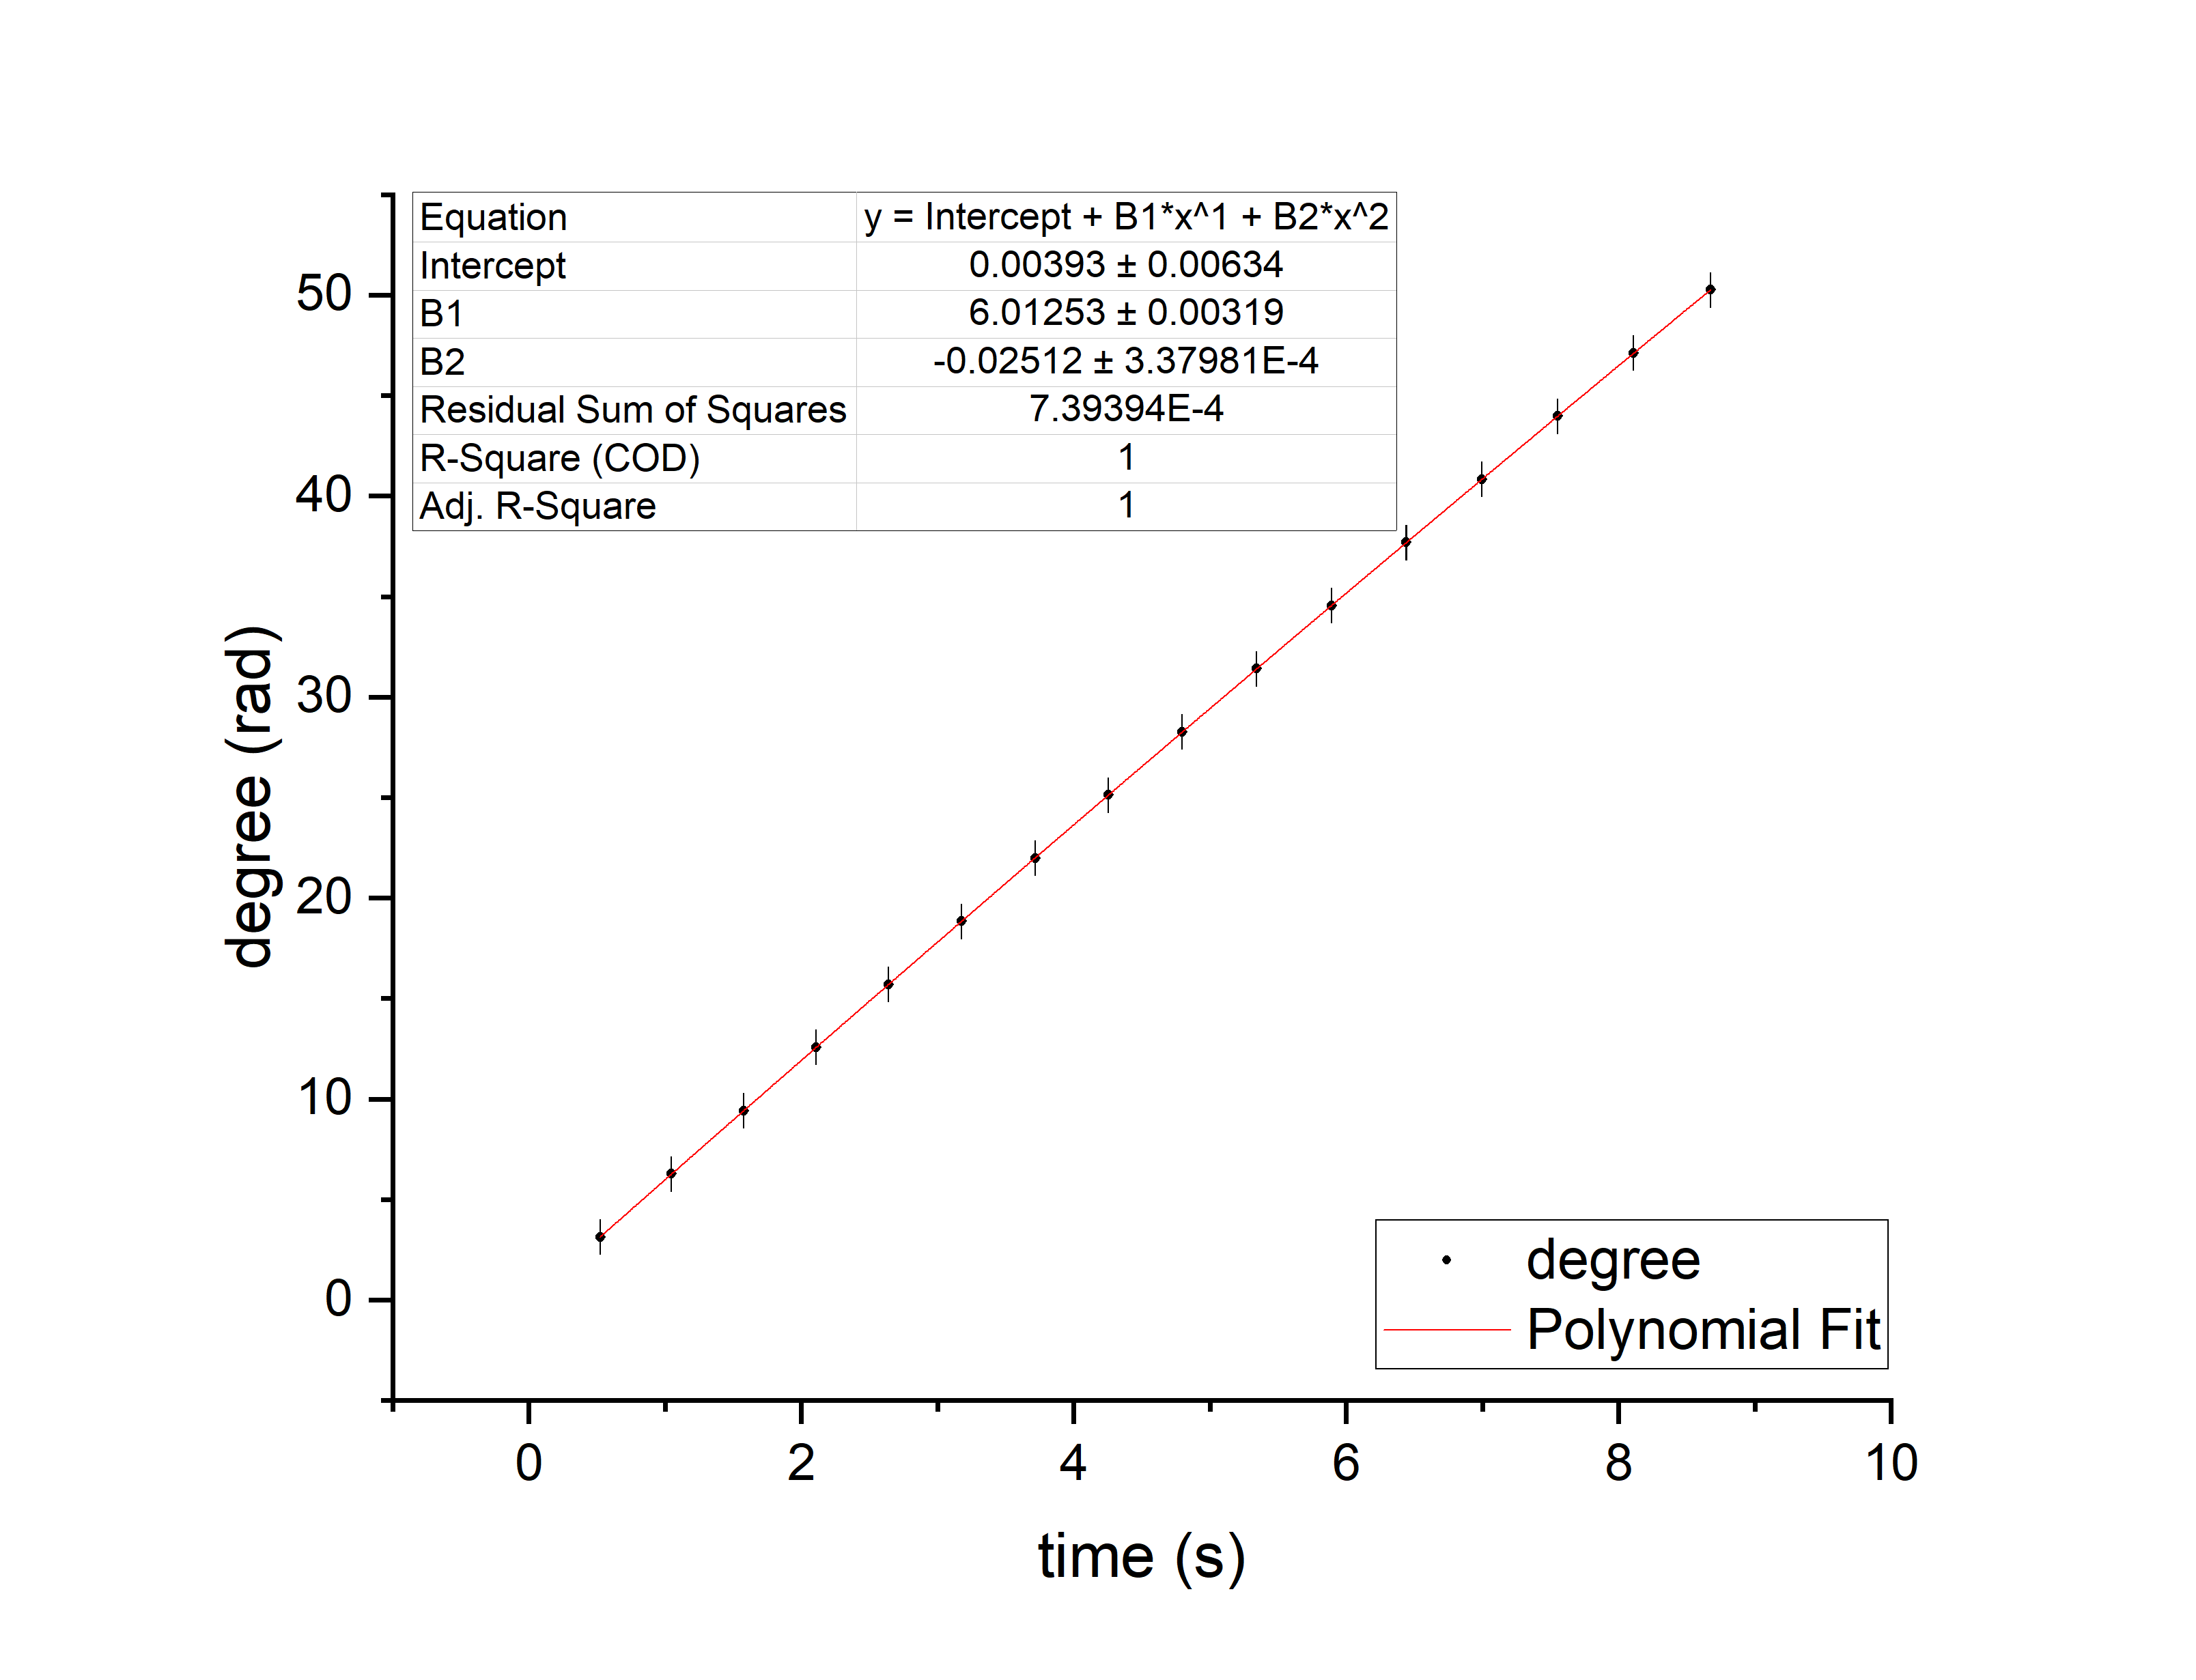
\includegraphics[width=12cm]{cirquewo.png}
    \caption{Time Measurement Data for Platform with Cirque and with weight}
\end{figure}

\begin{figure}[h]
    \centering
    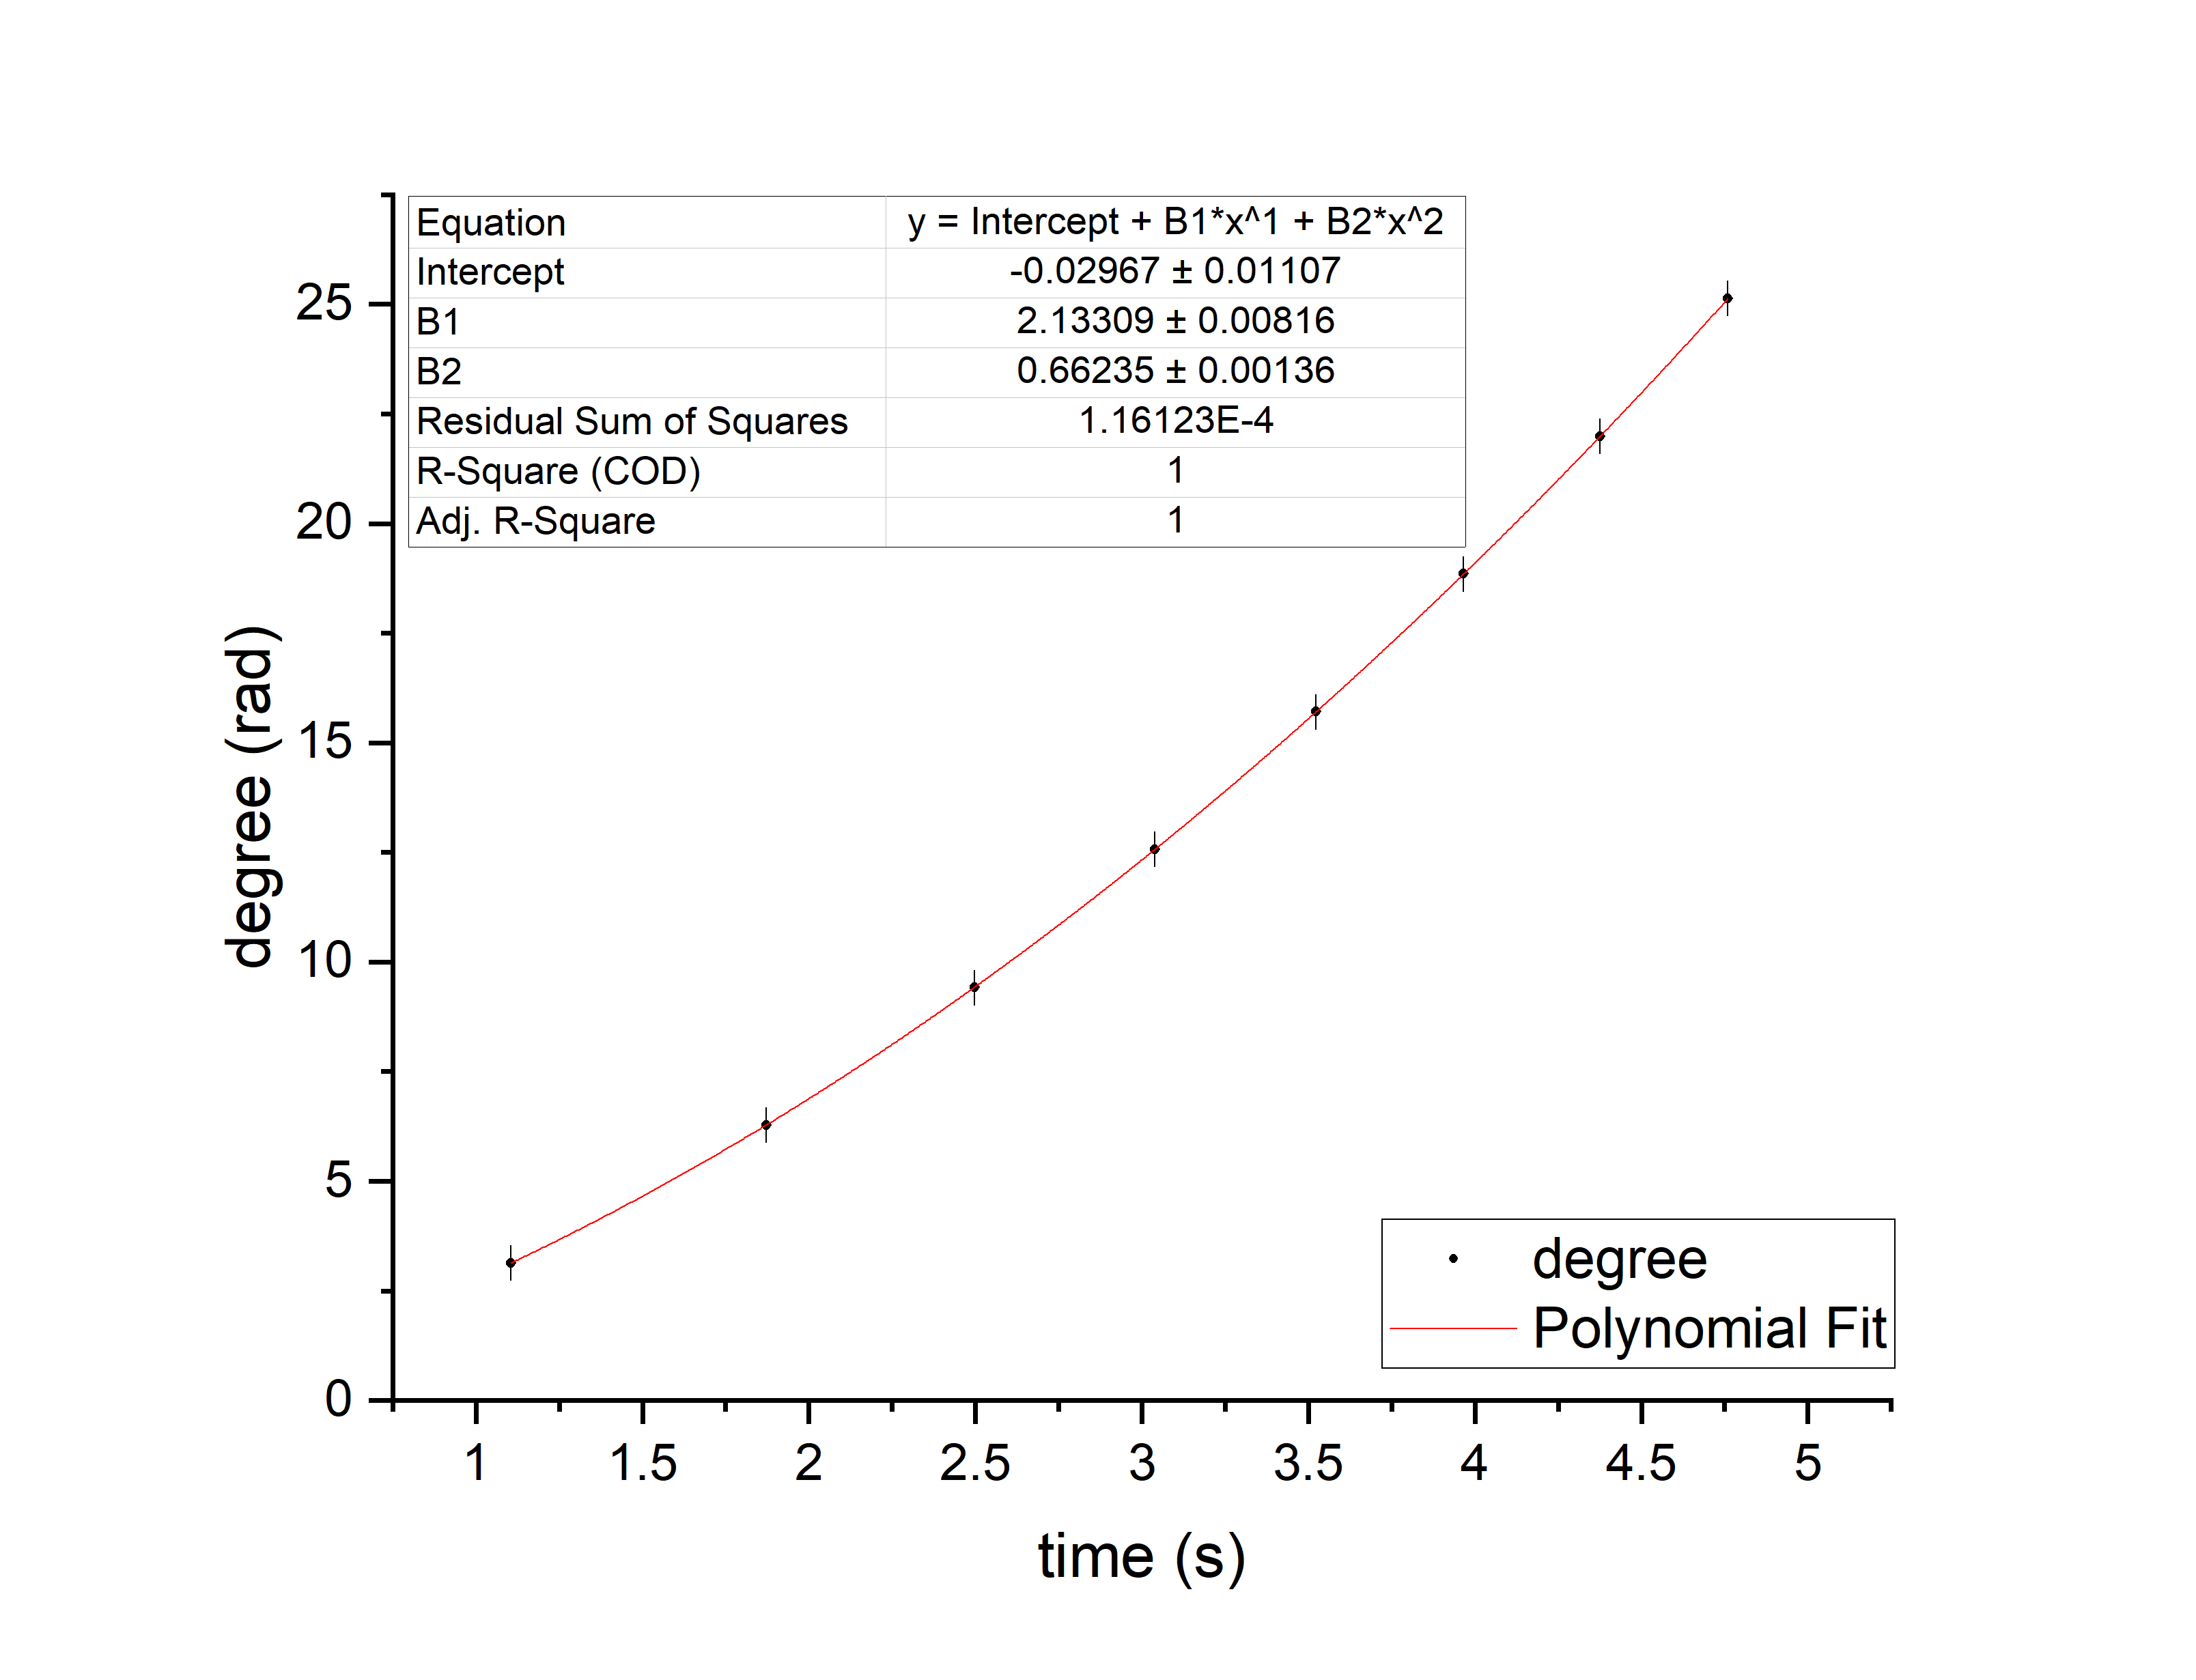
\includegraphics[width=12cm]{diskw.png}
    \caption{Time Measurement Data for Platform with Disk but without weight}
\end{figure}

\begin{figure}[h]
    \centering
    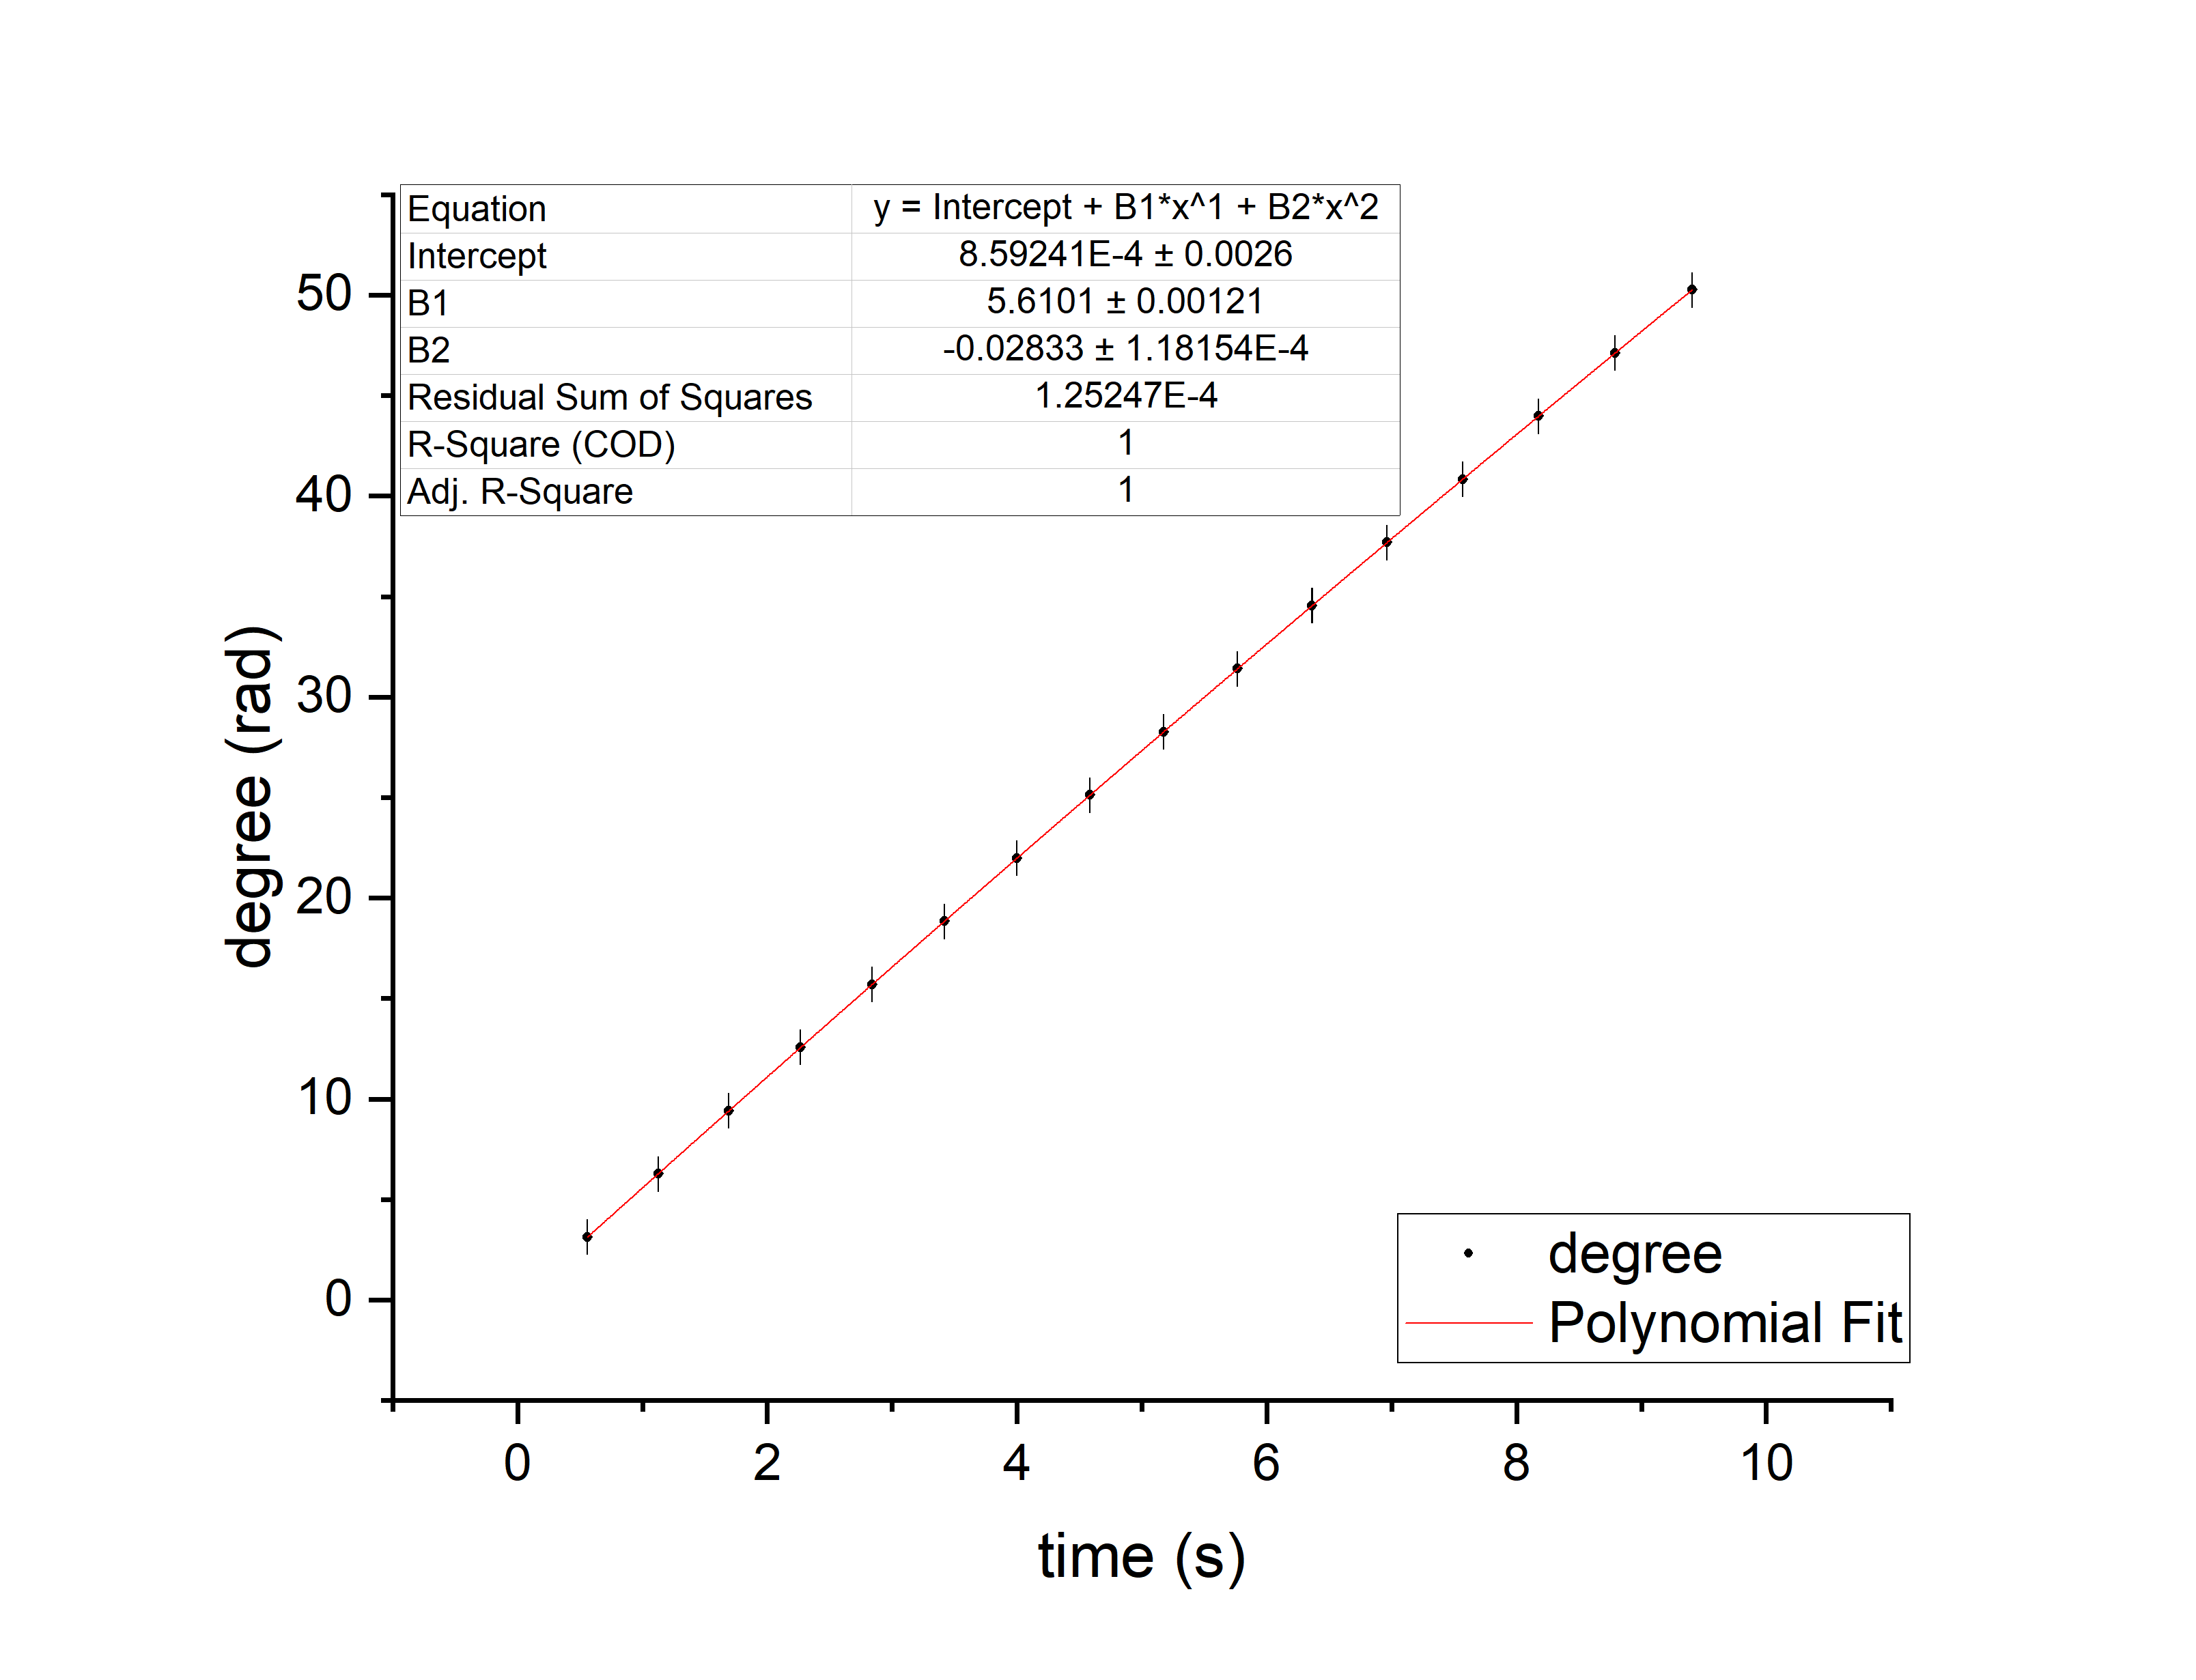
\includegraphics[width=12cm]{diskwo.png}
    \caption{Time Measurement Data for Platform with Disk and with weight}
\end{figure}

\begin{figure}[h]
    \centering
    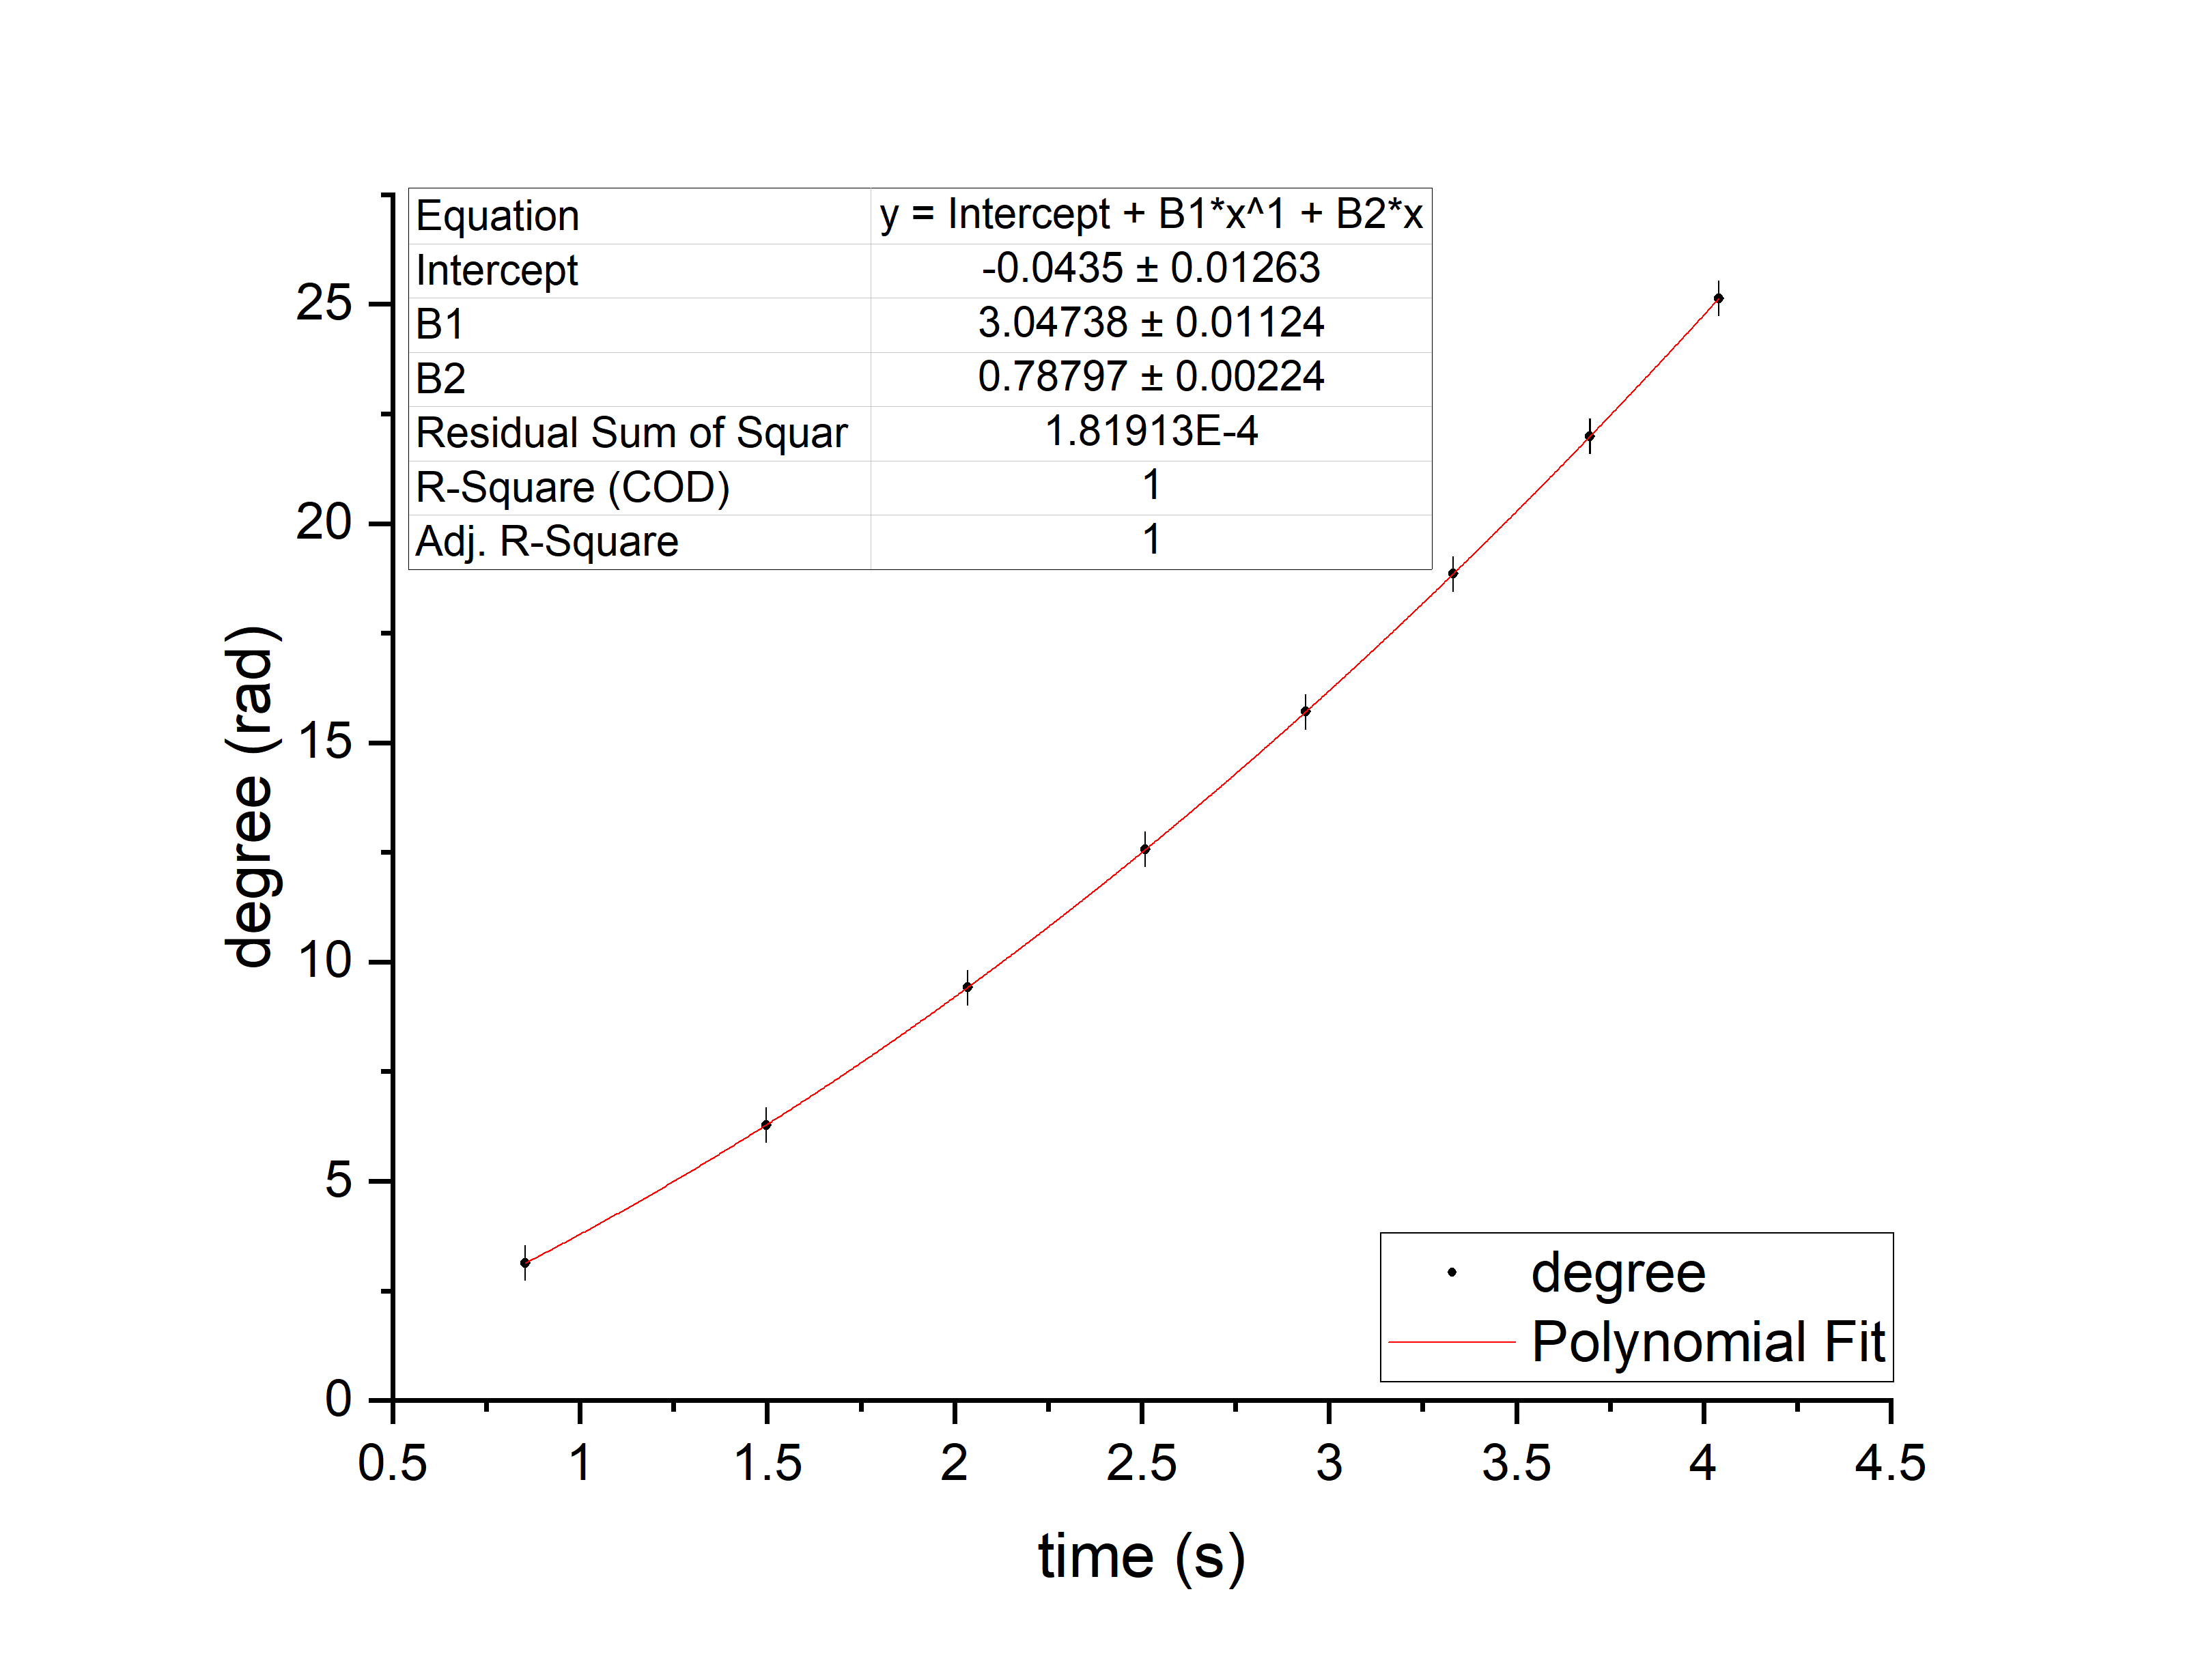
\includegraphics[width=12cm]{cylinderw.png}
    \caption{Time Measurement Data for Platform with Cylinders but without weight}
\end{figure}

\begin{figure}[h]
    \centering
    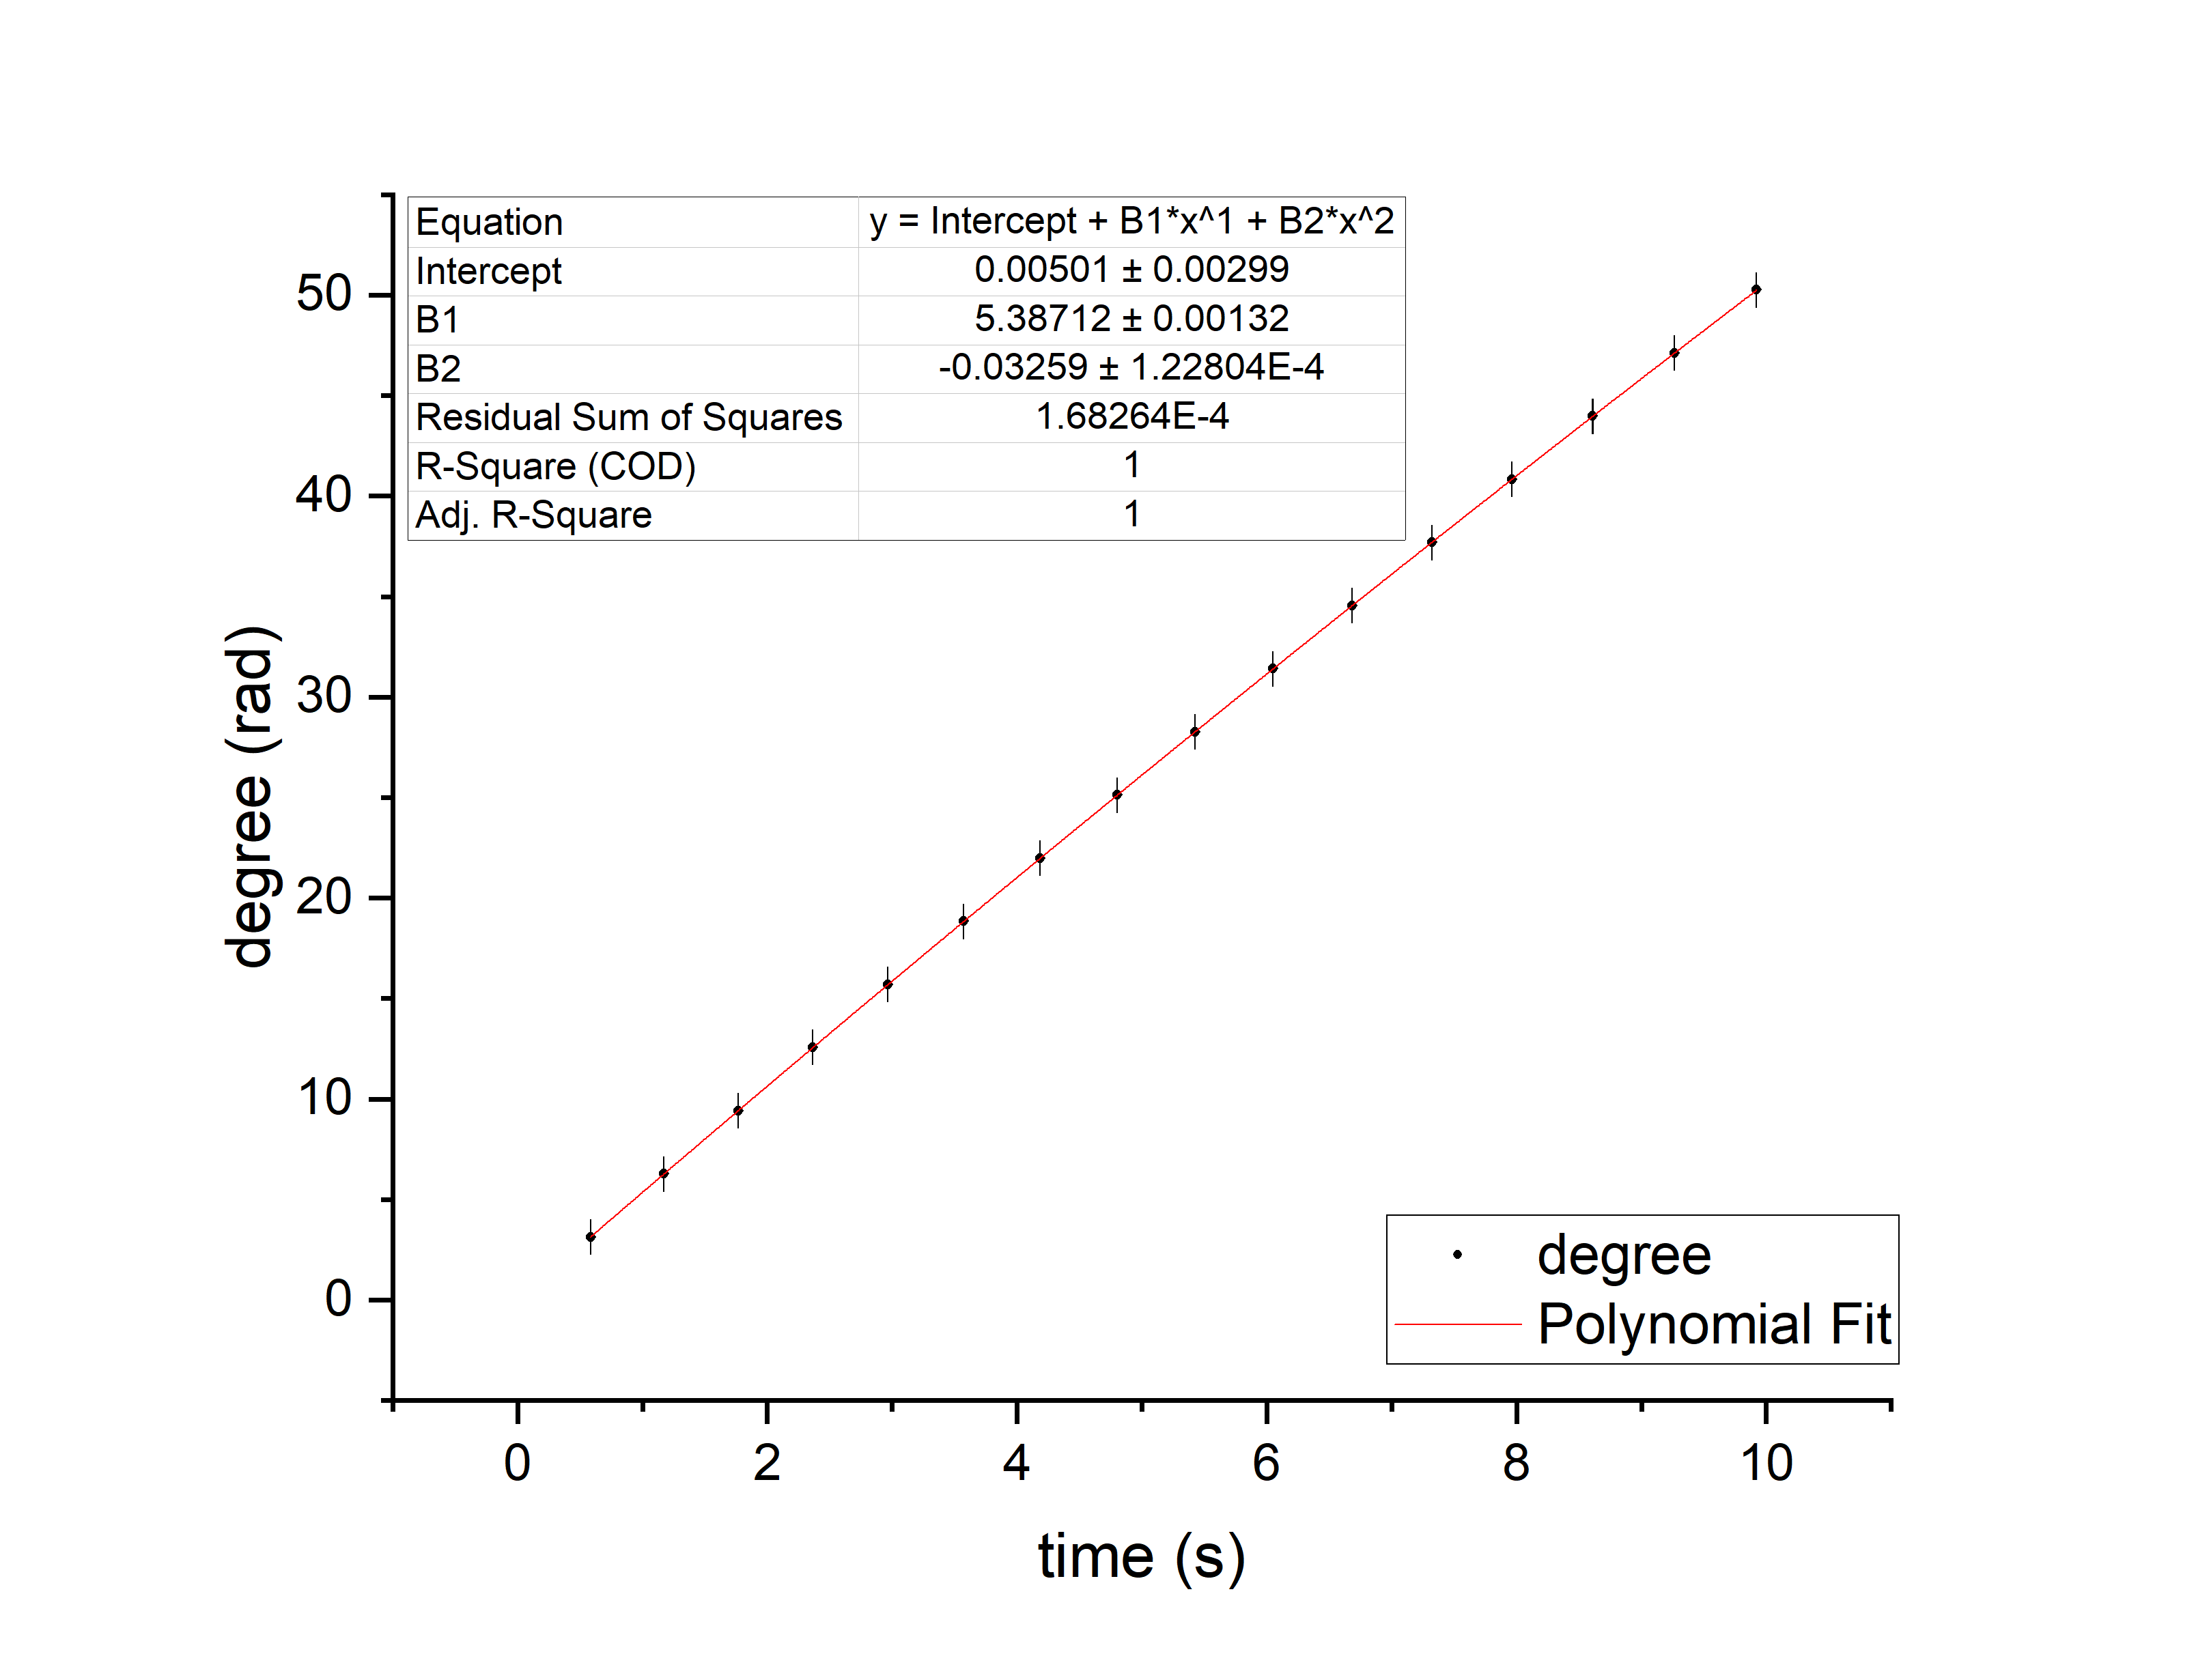
\includegraphics[width=12cm]{cylinderwo.png}
    \caption{Time Measurement Data for Platform with Cylinders and with weight}
\end{figure}



\end{document}